% Physiological Measurement submission, IOP Publishing template (iopjournal.cls, 2025 release,
% from publishingsupport.iopscience.iop.org). References: Harvard (author-year), as required by
% the journal. Supplementary material is compiled separately from supplementary_iop.tex.
\documentclass{iopjournal}

\usepackage{amssymb}
\usepackage{amsmath}
\usepackage{booktabs}
\usepackage{array}
\usepackage{multirow}
\usepackage{adjustbox}
\usepackage{makecell}
\usepackage{microtype}
\usepackage[round]{natbib}
\usepackage{placeins}
\usepackage{needspace}
\hypersetup{hidelinks}
\renewcommand{\topfraction}{0.9}
\renewcommand{\textfraction}{0.07}
\renewcommand{\floatpagefraction}{0.8}
\setcounter{topnumber}{3}

% running head without the template's placeholder journal details
\fancyhead[L]{\small Subject-independent surface EMG electrode reduction}
\fancyhead[C]{}
\fancyhead[R]{\small Ta \textit{et al}}

% kept so that generated tables compile; renders plain text
\newcommand{\rev}[1]{#1}

% Justified body text, abstract and captions (the class sets \raggedright globally).
\usepackage{ragged2e}
\AtBeginDocument{\justifying}
\makeatletter
\renewcommand{\@makecaption}[2]{\vskip\abovecaptionskip
\sbox\@tempboxa{\fontsize{8}{10}\selectfont {\bfseries #1.} #2}%
\ifdim \wd\@tempboxa >\hsize
{\justifying\fontsize{8}{10}\selectfont {\bfseries #1.} #2\par}
\else
\global \@minipagefalse
\hb@xt@\hsize{\hfil\box\@tempboxa\hfil}%
\fi
\vskip\belowcaptionskip}
\makeatother

% Revision marking (2026-09-23 editorial and statistical revision): revised text is shown in blue.
% Use \showchangesfalse for the clean submission PDF.
\newif\ifshowchanges
\showchangestrue
\ifdefined\cleanbuild \showchangesfalse \fi
\newcommand{\chg}[1]{\ifshowchanges{\color{blue}#1}\else{#1}\fi}

% AUTO-GENERATED by scripts/40_generate_macros.py - do not edit by hand.
% Every value is traceable via manuscript/generated/macro_provenance.csv

\newcommand{\GRABMyoParticipants}{43}
\newcommand{\GRABMyoSessions}{3}
\newcommand{\GRABMyoGestures}{17}
\newcommand{\GRABMyoActiveGestures}{16}
\newcommand{\GRABMyoWindows}{598{,}689}
\newcommand{\GRABMyoRecords}{15{,}351}
\newcommand{\GRABMyoRecordsFailed}{0}
\newcommand{\GRABMyoAgeMean}{26.4}
\newcommand{\GRABMyoAgeSD}{2.9}
\newcommand{\GRABMyoMale}{23}
\newcommand{\GRABMyoFemale}{20}
\newcommand{\GRABMyoCircMean}{24.1}
\newcommand{\GRABMyoCircSD}{2.3}
\newcommand{\GRABMyoArcSpacing}{3.0}
\newcommand{\GRABMyoActiveWindows}{563{,}472}
\newcommand{\FoldTrainingWindows}{550{,}368}
\newcommand{\TestWindowsPerParticipant}{13{,}104}
\newcommand{\DBFiveSubjects}{10}
\newcommand{\DBFiveAgeMean}{28.0}
\newcommand{\DBFiveAgeSD}{4.0}
\newcommand{\DBFiveMale}{8}
\newcommand{\DBFiveFemale}{2}
\newcommand{\DBFiveWindows}{21{,}089}
\newcommand{\GRABMyoFilesVerified}{30{,}715}
\newcommand{\FullRF}{0.502}
\newcommand{\FullRFLCB}{0.475}
\newcommand{\FullRFUCB}{0.528}
\newcommand{\FullRFSD}{0.090}
\newcommand{\FullRFMin}{0.346}
\newcommand{\FullRFMax}{0.670}
\newcommand{\FullSVM}{0.538}
\newcommand{\FullSVMLCB}{0.513}
\newcommand{\FullSVMUCB}{0.562}
\newcommand{\FullSVMSD}{0.085}
\newcommand{\FullSVMMin}{0.383}
\newcommand{\FullSVMMax}{0.718}
\newcommand{\FullXGB}{0.542}
\newcommand{\FullXGBLCB}{0.517}
\newcommand{\FullXGBUCB}{0.567}
\newcommand{\FullXGBSD}{0.085}
\newcommand{\FullXGBMin}{0.385}
\newcommand{\FullXGBMax}{0.702}
\newcommand{\KStarMarginPtOne}{14}
\newcommand{\KStarMarginPtTwo}{12}
\newcommand{\KStarMarginPtThree}{11}
\newcommand{\KStar}{12}
\newcommand{\KStarReductionPct}{25}
\newcommand{\SVMvsRFDiff}{+0.0362}
\newcommand{\SVMvsRFLCB}{+0.0284}
\newcommand{\SVMvsRFUCB}{+0.0444}
\newcommand{\SVMvsRFW}{15.0}
\newcommand{\SVMvsRFP}{< 0.001}
\newcommand{\SVMvsRFR}{+0.97}
\newcommand{\XGBvsRFDiff}{+0.0408}
\newcommand{\XGBvsRFLCB}{+0.0340}
\newcommand{\XGBvsRFUCB}{+0.0475}
\newcommand{\XGBvsRFW}{10.0}
\newcommand{\XGBvsRFP}{< 0.001}
\newcommand{\XGBvsRFR}{+0.98}
\newcommand{\XGBvsSVMDiff}{+0.0045}
\newcommand{\XGBvsSVMLCB}{-0.0015}
\newcommand{\XGBvsSVMUCB}{+0.0107}
\newcommand{\XGBvsSVMW}{354.0}
\newcommand{\XGBvsSVMP}{= 0.154}
\newcommand{\XGBvsSVMR}{+0.25}
\newcommand{\SVMCalibTwentyK}{0.555}
\newcommand{\SVMCalibFortyK}{0.591}
\newcommand{\CurveKSixteen}{0.541}
\newcommand{\CurveKSixteenSD}{0.084}
\newcommand{\CurveKFourteen}{0.535}
\newcommand{\CurveKFourteenSD}{0.083}
\newcommand{\DeltaKFourteen}{-0.0060}
\newcommand{\DeltaKFourteenLCB}{-0.0081}
\newcommand{\DeltaKFourteenUCB}{-0.0039}
\newcommand{\CurveKThirteen}{0.530}
\newcommand{\CurveKThirteenSD}{0.083}
\newcommand{\DeltaKThirteen}{-0.0109}
\newcommand{\DeltaKThirteenLCB}{-0.0133}
\newcommand{\DeltaKThirteenUCB}{-0.0085}
\newcommand{\CurveKTwelve}{0.528}
\newcommand{\CurveKTwelveSD}{0.084}
\newcommand{\DeltaKTwelve}{-0.0133}
\newcommand{\DeltaKTwelveLCB}{-0.0160}
\newcommand{\DeltaKTwelveUCB}{-0.0106}
\newcommand{\CurveKEleven}{0.521}
\newcommand{\CurveKElevenSD}{0.084}
\newcommand{\DeltaKEleven}{-0.0204}
\newcommand{\DeltaKElevenLCB}{-0.0246}
\newcommand{\DeltaKElevenUCB}{-0.0162}
\newcommand{\CurveKTen}{0.515}
\newcommand{\CurveKTenSD}{0.083}
\newcommand{\DeltaKTen}{-0.0259}
\newcommand{\DeltaKTenLCB}{-0.0311}
\newcommand{\DeltaKTenUCB}{-0.0205}
\newcommand{\CurveKEight}{0.505}
\newcommand{\CurveKEightSD}{0.085}
\newcommand{\DeltaKEight}{-0.0366}
\newcommand{\DeltaKEightLCB}{-0.0440}
\newcommand{\DeltaKEightUCB}{-0.0289}
\newcommand{\CurveKSix}{0.480}
\newcommand{\CurveKSixSD}{0.084}
\newcommand{\DeltaKSix}{-0.0610}
\newcommand{\DeltaKSixLCB}{-0.0713}
\newcommand{\DeltaKSixUCB}{-0.0507}
\newcommand{\CurveKFour}{0.397}
\newcommand{\CurveKFourSD}{0.071}
\newcommand{\DeltaKFour}{-0.1444}
\newcommand{\DeltaKFourLCB}{-0.1590}
\newcommand{\DeltaKFourUCB}{-0.1306}
\newcommand{\CurveKTwo}{0.299}
\newcommand{\CurveKTwoSD}{0.057}
\newcommand{\DeltaKTwo}{-0.2420}
\newcommand{\DeltaKTwoLCB}{-0.2603}
\newcommand{\DeltaKTwoUCB}{-0.2230}
\newcommand{\CurveKOne}{0.181}
\newcommand{\CurveKOneSD}{0.040}
\newcommand{\DeltaKOne}{-0.3603}
\newcommand{\DeltaKOneLCB}{-0.3832}
\newcommand{\DeltaKOneUCB}{-0.3369}
\newcommand{\CurveTrainWindows}{200{,}000}
\newcommand{\LambdaCurveMaxSpread}{0.0040}
\newcommand{\TopFourSet}{4, 6, 7, 14}
\newcommand{\TopFourFolds}{36}
\newcommand{\DroppedFourSet}{9, 11, 12, 16}
\newcommand{\DroppedFourFolds}{43}
\newcommand{\TopFourShare}{34.0}
\newcommand{\BottomEightShare}{39.6}
\newcommand{\UOverAMedian}{2.4}
\newcommand{\UOverAMax}{9.4}
\newcommand{\TopTwelveDiffersLambdaPtTwoFive}{0}
\newcommand{\TopTwelveDiffersLambdaPtFive}{0}
\newcommand{\TopTwelveDiffersLambdaOne}{1}
\newcommand{\HTwoKFourDiff}{+0.0172}
\newcommand{\HTwoKFourLCB}{+0.0071}
\newcommand{\HTwoKFourUCB}{+0.0274}
\newcommand{\HTwoKFourP}{= 0.007}
\newcommand{\HTwoKFourR}{+0.50}
\newcommand{\HTwoKSixDiff}{+0.0370}
\newcommand{\HTwoKSixLCB}{+0.0286}
\newcommand{\HTwoKSixUCB}{+0.0452}
\newcommand{\HTwoKSixP}{< 0.001}
\newcommand{\HTwoKSixR}{+0.92}
\newcommand{\HTwoKEightDiff}{+0.0243}
\newcommand{\HTwoKEightLCB}{+0.0176}
\newcommand{\HTwoKEightUCB}{+0.0308}
\newcommand{\HTwoKEightP}{< 0.001}
\newcommand{\HTwoKEightR}{+0.86}
\newcommand{\HTwoKTwelveDiff}{+0.0074}
\newcommand{\HTwoKTwelveLCB}{+0.0046}
\newcommand{\HTwoKTwelveUCB}{+0.0103}
\newcommand{\HTwoKTwelveP}{< 0.001}
\newcommand{\HTwoKTwelveR}{+0.71}
\newcommand{\HTwoAllSig}{yes}
\newcommand{\PctKFour}{65}
\newcommand{\PctKAboveNinetyFiveFour}{3}
\newcommand{\PctKSix}{89}
\newcommand{\PctKAboveNinetyFiveSix}{11}
\newcommand{\PctKEight}{82}
\newcommand{\PctKAboveNinetyFiveEight}{6}
\newcommand{\PctKTwelve}{66}
\newcommand{\PctKAboveNinetyFiveTwelve}{1}
\newcommand{\VSPermKFourDiff}{-0.0018}
\newcommand{\VSPermKFourP}{= 0.678}
\newcommand{\VSGeomKFourDiff}{-0.0005}
\newcommand{\VSGeomKFourP}{= 0.986}
\newcommand{\VSMiKFourDiff}{+0.1031}
\newcommand{\VSMiKFourP}{< 0.001}
\newcommand{\VSPermKSixDiff}{+0.0126}
\newcommand{\VSPermKSixP}{= 0.009}
\newcommand{\VSGeomKSixDiff}{+0.0341}
\newcommand{\VSGeomKSixP}{< 0.001}
\newcommand{\VSMiKSixDiff}{+0.0934}
\newcommand{\VSMiKSixP}{< 0.001}
\newcommand{\VSPermKEightDiff}{+0.0033}
\newcommand{\VSPermKEightP}{= 0.069}
\newcommand{\VSGeomKEightDiff}{+0.0047}
\newcommand{\VSGeomKEightP}{= 0.267}
\newcommand{\VSMiKEightDiff}{+0.0737}
\newcommand{\VSMiKEightP}{< 0.001}
\newcommand{\VSPermKTwelveDiff}{+0.0001}
\newcommand{\VSPermKTwelveP}{= 0.995}
\newcommand{\VSGeomKTwelveDiff}{+0.0070}
\newcommand{\VSGeomKTwelveP}{= 0.058}
\newcommand{\VSMiKTwelveDiff}{+0.0051}
\newcommand{\VSMiKTwelveP}{= 0.007}
\newcommand{\HThreeMaxAbsDiff}{0.0015}
\newcommand{\HThreeNSig}{0}
\newcommand{\HThreeNTests}{12}
\newcommand{\HThreeMinP}{= 0.216}
\newcommand{\HThreeMinTied}{36}
\newcommand{\FaithProtocolCells}{172}
\newcommand{\FaithProtocolMeanDiff}{0.0014}
\newcommand{\FaithProtocolMaxDiff}{0.0084}
\newcommand{\FaithTopKTwo}{0.263}
\newcommand{\FaithBottomKTwo}{0.292}
\newcommand{\FaithTopKFour}{0.351}
\newcommand{\FaithRandomKFour}{0.366}
\newcommand{\FaithBottomKFour}{0.382}
\newcommand{\FaithTopKSix}{0.376}
\newcommand{\FaithRandomKSix}{0.416}
\newcommand{\FaithBottomKSix}{0.454}
\newcommand{\FaithTopKEight}{0.408}
\newcommand{\FaithRandomKEight}{0.445}
\newcommand{\FaithBottomKEight}{0.469}
\newcommand{\FaithTopKTen}{0.445}
\newcommand{\FaithBottomKTen}{0.475}
\newcommand{\FaithTopKTwelve}{0.455}
\newcommand{\FaithRandomKTwelve}{0.478}
\newcommand{\FaithBottomKTwelve}{0.485}
\newcommand{\FaithTopKFourteen}{0.487}
\newcommand{\FaithBottomKFourteen}{0.491}
\newcommand{\FaithTBKTwoDiff}{-0.0297}
\newcommand{\FaithTBKTwoLCB}{-0.0419}
\newcommand{\FaithTBKTwoUCB}{-0.0166}
\newcommand{\FaithTBKTwoP}{< 0.001}
\newcommand{\FaithTBKFourDiff}{-0.0314}
\newcommand{\FaithTBKFourLCB}{-0.0447}
\newcommand{\FaithTBKFourUCB}{-0.0177}
\newcommand{\FaithTBKFourP}{< 0.001}
\newcommand{\FaithTRKFourDiff}{-0.0151}
\newcommand{\FaithTRKFourLCB}{-0.0239}
\newcommand{\FaithTRKFourUCB}{-0.0061}
\newcommand{\FaithTRKFourP}{= 0.010}
\newcommand{\FaithRBKFourDiff}{-0.0163}
\newcommand{\FaithRBKFourLCB}{-0.0265}
\newcommand{\FaithRBKFourUCB}{-0.0061}
\newcommand{\FaithRBKFourP}{= 0.013}
\newcommand{\FaithTBKSixDiff}{-0.0775}
\newcommand{\FaithTBKSixLCB}{-0.0921}
\newcommand{\FaithTBKSixUCB}{-0.0627}
\newcommand{\FaithTBKSixP}{< 0.001}
\newcommand{\FaithTRKSixDiff}{-0.0398}
\newcommand{\FaithTRKSixLCB}{-0.0487}
\newcommand{\FaithTRKSixUCB}{-0.0307}
\newcommand{\FaithTRKSixP}{< 0.001}
\newcommand{\FaithRBKSixDiff}{-0.0377}
\newcommand{\FaithRBKSixLCB}{-0.0459}
\newcommand{\FaithRBKSixUCB}{-0.0293}
\newcommand{\FaithRBKSixP}{< 0.001}
\newcommand{\FaithTBKEightDiff}{-0.0618}
\newcommand{\FaithTBKEightLCB}{-0.0772}
\newcommand{\FaithTBKEightUCB}{-0.0461}
\newcommand{\FaithTBKEightP}{< 0.001}
\newcommand{\FaithTRKEightDiff}{-0.0377}
\newcommand{\FaithTRKEightLCB}{-0.0476}
\newcommand{\FaithTRKEightUCB}{-0.0273}
\newcommand{\FaithTRKEightP}{< 0.001}
\newcommand{\FaithRBKEightDiff}{-0.0242}
\newcommand{\FaithRBKEightLCB}{-0.0309}
\newcommand{\FaithRBKEightUCB}{-0.0172}
\newcommand{\FaithRBKEightP}{< 0.001}
\newcommand{\FaithTBKTenDiff}{-0.0297}
\newcommand{\FaithTBKTenLCB}{-0.0399}
\newcommand{\FaithTBKTenUCB}{-0.0188}
\newcommand{\FaithTBKTenP}{< 0.001}
\newcommand{\FaithTBKTwelveDiff}{-0.0302}
\newcommand{\FaithTBKTwelveLCB}{-0.0385}
\newcommand{\FaithTBKTwelveUCB}{-0.0218}
\newcommand{\FaithTBKTwelveP}{< 0.001}
\newcommand{\FaithTRKTwelveDiff}{-0.0228}
\newcommand{\FaithTRKTwelveLCB}{-0.0296}
\newcommand{\FaithTRKTwelveUCB}{-0.0158}
\newcommand{\FaithTRKTwelveP}{< 0.001}
\newcommand{\FaithRBKTwelveDiff}{-0.0074}
\newcommand{\FaithRBKTwelveLCB}{-0.0101}
\newcommand{\FaithRBKTwelveUCB}{-0.0046}
\newcommand{\FaithRBKTwelveP}{< 0.001}
\newcommand{\FaithTBKFourteenDiff}{-0.0038}
\newcommand{\FaithTBKFourteenLCB}{-0.0084}
\newcommand{\FaithTBKFourteenUCB}{+0.0009}
\newcommand{\FaithTBKFourteenP}{= 0.150}
\newcommand{\FaithNTests}{15}
\newcommand{\FaithNSig}{14}
\newcommand{\FaithTBAllSig}{no}
\newcommand{\StabSubjPairs}{903}
\newcommand{\StabSubjRho}{0.927}
\newcommand{\StabSubjRhoSD}{0.038}
\newcommand{\StabSubjJacFour}{0.752}
\newcommand{\StabSubjJacSix}{0.905}
\newcommand{\StabSubjJacEight}{0.803}
\newcommand{\StabInnerPairs}{430}
\newcommand{\StabInnerRho}{0.948}
\newcommand{\StabInnerRhoSD}{0.021}
\newcommand{\StabInnerJacFour}{0.816}
\newcommand{\StabInnerJacSix}{0.992}
\newcommand{\StabInnerJacEight}{0.838}
\newcommand{\StabOuterPairs}{903}
\newcommand{\StabOuterRho}{0.987}
\newcommand{\StabOuterRhoSD}{0.008}
\newcommand{\StabOuterJacFour}{0.888}
\newcommand{\StabOuterJacSix}{1.000}
\newcommand{\StabOuterJacEight}{0.923}
\newcommand{\CSOneSOne}{0.492}
\newcommand{\CSOneSOneSD}{0.101}
\newcommand{\CSOneSOneTrain}{183{,}456}
\newcommand{\CSOneSTwo}{0.528}
\newcommand{\CSOneSTwoSD}{0.088}
\newcommand{\CSOneSTwoTrain}{183{,}456}
\newcommand{\CSOneSThree}{0.510}
\newcommand{\CSOneSThreeSD}{0.090}
\newcommand{\CSOneSThreeTrain}{183{,}456}
\newcommand{\CSTwoSThree}{0.530}
\newcommand{\CSTwoSThreeSD}{0.095}
\newcommand{\CSTwoSThreeTrain}{366{,}912}
\newcommand{\CSSTwoVsSOneDiff}{+0.0355}
\newcommand{\CSSTwoVsSOneLCB}{+0.0091}
\newcommand{\CSSTwoVsSOneUCB}{+0.0621}
\newcommand{\CSSTwoVsSOneW}{287.0}
\newcommand{\CSSTwoVsSOneP}{= 0.024}
\newcommand{\CSSThreeVsSOneDiff}{+0.0172}
\newcommand{\CSSThreeVsSOneLCB}{-0.0038}
\newcommand{\CSSThreeVsSOneUCB}{+0.0391}
\newcommand{\CSSThreeVsSOneW}{381.0}
\newcommand{\CSSThreeVsSOneP}{= 0.272}
\newcommand{\CSTwoVsOneDiff}{+0.0210}
\newcommand{\CSTwoVsOneLCB}{+0.0146}
\newcommand{\CSTwoVsOneUCB}{+0.0274}
\newcommand{\CSTwoVsOneW}{77.0}
\newcommand{\CSTwoVsOneP}{< 0.001}
\newcommand{\DBFiveFull}{0.281}
\newcommand{\DBFiveFullSD}{0.099}
\newcommand{\DBFiveFullMin}{0.096}
\newcommand{\DBFiveFullMax}{0.386}
\newcommand{\DBFiveKSixteen}{0.281}
\newcommand{\DBFiveKSixteenSD}{0.099}
\newcommand{\DBFiveKTwelve}{0.268}
\newcommand{\DBFiveKTwelveSD}{0.092}
\newcommand{\DBFiveKEight}{0.252}
\newcommand{\DBFiveKEightSD}{0.068}
\newcommand{\DBFiveKFour}{0.180}
\newcommand{\DBFiveKFourSD}{0.026}
\newcommand{\DBFiveDeltaKEleven}{-0.0211}
\newcommand{\DBFiveDeltaKElevenLCB}{-0.03412}
\newcommand{\DBFiveDeltaKTwelve}{-0.0126}
\newcommand{\DBFiveDeltaKTwelveLCB}{-0.01999}
\newcommand{\DBFiveDeltaKThirteen}{-0.0143}
\newcommand{\DBFiveDeltaKThirteenLCB}{-0.03119}
\newcommand{\DBFiveDeltaKFourteen}{-0.0119}
\newcommand{\DBFiveDeltaKFourteenLCB}{-0.02744}
\newcommand{\DBFiveDeltaKFifteen}{-0.0108}
\newcommand{\DBFiveDeltaKFifteenLCB}{-0.02377}
\newcommand{\DBFiveKStarMarginPtOne}{none}
\newcommand{\DBFiveKStarMarginPtTwo}{12}
\newcommand{\DBFiveKStarMarginPtThree}{12}
\newcommand{\DBFiveNIPassing}{12}
\newcommand{\DBFiveSeedFrac}{95.5}
\newcommand{\DBFiveSeedN}{200}
\newcommand{\DBFiveSeedHits}{191}
\newcommand{\DBFiveSeedLCBMin}{-0.0201}
\newcommand{\DBFiveSeedLCBMax}{-0.0195}
\newcommand{\BipFull}{0.478}
\newcommand{\BipFullSD}{0.089}
\newcommand{\BipKOne}{0.174}
\newcommand{\BipKOneSD}{0.044}
\newcommand{\BipKTwo}{0.240}
\newcommand{\BipKTwoSD}{0.049}
\newcommand{\BipKThree}{0.310}
\newcommand{\BipKThreeSD}{0.070}
\newcommand{\BipKFour}{0.356}
\newcommand{\BipKFourSD}{0.080}
\newcommand{\BipKFive}{0.405}
\newcommand{\BipKFiveSD}{0.085}
\newcommand{\BipKSix}{0.442}
\newcommand{\BipKSixSD}{0.086}
\newcommand{\BipKSeven}{0.464}
\newcommand{\BipKSevenSD}{0.085}
\newcommand{\BipKEight}{0.480}
\newcommand{\BipKEightSD}{0.089}
\newcommand{\BipDeltaKOne}{-0.3052}
\newcommand{\BipDeltaKOneLCB}{-0.3298}
\newcommand{\BipDeltaKTwo}{-0.2399}
\newcommand{\BipDeltaKTwoLCB}{-0.2615}
\newcommand{\BipDeltaKThree}{-0.1697}
\newcommand{\BipDeltaKThreeLCB}{-0.1852}
\newcommand{\BipDeltaKFour}{-0.1240}
\newcommand{\BipDeltaKFourLCB}{-0.1392}
\newcommand{\BipDeltaKFive}{-0.0742}
\newcommand{\BipDeltaKFiveLCB}{-0.0845}
\newcommand{\BipDeltaKSix}{-0.0375}
\newcommand{\BipDeltaKSixLCB}{-0.0451}
\newcommand{\BipDeltaKSeven}{-0.0158}
\newcommand{\BipDeltaKSevenLCB}{-0.0203}
\newcommand{\BipKStarMarginPtOne}{none}
\newcommand{\BipKStarMarginPtTwo}{none}
\newcommand{\BipKStarMarginPtThree}{7}
\newcommand{\BipSeedFracSeven}{0}
\newcommand{\BipSeedHitsSeven}{0}
\newcommand{\BipSeedN}{200}
\newcommand{\BipSeedLCBMaxSeven}{-0.0203}
\newcommand{\BipSeedLCBMinSeven}{-0.0207}
\newcommand{\BipCurveRefK}{0.480}
\newcommand{\BipTopThreeSet}{5, 6, 7}
\newcommand{\BipTopThreeFolds}{30}
\newcommand{\FixedDev}{22}
\newcommand{\FixedTest}{21}
\newcommand{\FixedChannels}{1, 2, 4, 5, 6, 7, 8, 10, 13, 14, 15, 16}
\newcommand{\FixedDropped}{3, 9, 11, 12}
\newcommand{\FixedFull}{0.522}
\newcommand{\FixedTwelve}{0.510}
\newcommand{\FixedDiff}{-0.0124}
\newcommand{\FixedLCB}{-0.0179}
\newcommand{\FixedUCB}{-0.0077}
\newcommand{\FixedLamZeroSame}{yes}
\newcommand{\FixedNLambdaSameOrig}{4}
\newcommand{\FixedSwapDev}{21}
\newcommand{\FixedSwapTest}{22}
\newcommand{\FixedSwapDropped}{9, 11, 12, 13}
\newcommand{\FixedSwapNLambdaSame}{4}
\newcommand{\FixedSwapFull}{0.529}
\newcommand{\FixedSwapTwelve}{0.516}
\newcommand{\FixedSwapDiff}{-0.0135}
\newcommand{\FixedSwapLCBSix}{-0.020020}
\newcommand{\FixedSwapUCB}{-0.0066}
\newcommand{\FixedSwapNI}{no}
\newcommand{\FixedDroppedBoth}{9, 11, 12}
\newcommand{\FixedDroppedBothN}{3}
\newcommand{\RedundDiff}{-0.0005}
\newcommand{\RedundLCB}{-0.0021}
\newcommand{\RedundUCB}{+0.0010}
\newcommand{\RedundRho}{0.994}
\newcommand{\RedundTopTwelveSame}{34}
\newcommand{\KStarHolmPtOne}{14}
\newcommand{\KStarFixSeqPtOne}{14}
\newcommand{\KStarHolm}{12}
\newcommand{\KStarFixSeq}{12}
\newcommand{\KStarHolmPtThree}{11}
\newcommand{\KStarFixSeqPtThree}{11}
\newcommand{\HolmPKTwelve}{= 0.002}
\newcommand{\HolmPKEleven}{= 1.000}
\newcommand{\HolmSameAllLambda}{yes}
\newcommand{\DBFiveKStarHolmPtOne}{none}
\newcommand{\DBFiveKStarHolmPtTwo}{none}
\newcommand{\DBFiveKStarHolmPtThree}{12}
\newcommand{\DBFiveDeltaKTwelveLCBSix}{-0.019994}
\newcommand{\MarginPctOfRef}{3.7}
\newcommand{\MarginPctAboveChance}{4.2}
\newcommand{\LOOMonoFolds}{43}
\newcommand{\LOOMonoIdentical}{43}
\newcommand{\LOOMonoInProbe}{6}
\newcommand{\LOODBFiveFolds}{10}
\newcommand{\LOODBFiveIdentical}{10}
\newcommand{\LOODBFiveInProbe}{10}
\newcommand{\LOOBipFolds}{43}
\newcommand{\LOOBipIdentical}{43}
\newcommand{\LOOBipInProbe}{6}
\newcommand{\LOOMonoMin}{8.52}
\newcommand{\LOOMonoMax}{9.45}
\newcommand{\LOOBipPooled}{3.40}
\newcommand{\LOOBipRule}{4}
\newcommand{\HTwoSameKFour}{40}
\newcommand{\HTwoSameKSix}{43}
\newcommand{\HTwoSameKEight}{40}
\newcommand{\HTwoSameKTwelve}{43}


\begin{document}

\title{Subject-independent surface EMG electrode reduction using cross-fitted attribution: a prespecified non-inferiority study}

\author{Minh-Tri Ta$^1$, Hoang-Khang Phan$^{2,3}$ and Le-Giang Tran$^{4,*}$}

\affil{$^1$College of Engineering and Computer Science, VinUniversity, Hanoi, Vietnam}

\affil{$^2$Department of Biomedical Engineering, Faculty of Applied Science, Ho Chi Minh City University of Technology (HCMUT), 268 Ly Thuong Kiet Street, District 10, Ho Chi Minh City, Vietnam}

\affil{$^3$Vietnam National University Ho Chi Minh City, Linh Trung Ward, Thu Duc City, Ho Chi Minh City, Vietnam}

\affil{$^4$Faculty of Electronics Technology, Industrial University of Ho Chi Minh City, Ho Chi Minh City, Vietnam}

\affil{$^*$Author to whom any correspondence should be addressed.}

\email{tranlegiang@iuh.edu.vn}

\keywords{surface electromyography, gesture recognition, electrode selection, SHAP, cross-fitting, non-inferiority, leave-one-subject-out}

\begin{abstract}
\justifying
\textit{Objective.} Reducing the number of surface electromyography (sEMG) electrodes can simplify wearable interfaces, but only if recognition performance is preserved for previously unseen users. We investigated whether attribution-guided electrode selection could reduce a forearm sEMG array without meaningful loss of subject-independent gesture recognition.
\textit{Approach.} We analysed 43 GRABMyo participants using 16 monopolar forearm electrodes and 16 active gestures. All analyses followed a leave-one-subject-out design in which the test participant was excluded from feature standardisation, model fitting and electrode ranking. Electrode importance was estimated with TreeSHAP \chg{using} participant-disjoint cross-fitting, and reduced models were retrained on the highest-ranked electrodes. Performance was compared with the full array against a prespecified non-inferiority margin of 0.02 Macro-F1, using participant-level cluster-bootstrap confidence intervals (CI). \chg{Secondary analyses compared attribution with random selection, tested a stability penalty and applied deletion with retraining.}
\textit{Main results.} The full array achieved a Macro-F1 of \FullXGB\ (95\% CI \FullXGBLCB--\FullXGBUCB). The smallest non-inferior subset contained \KStar\ electrodes (mean difference $\DeltaKTwelve$, 95\% CI $\DeltaKTwelveLCB$ to $\DeltaKTwelveUCB$); \chg{eleven did not.} Attribution-ranked subsets outperformed the mean random-subset baseline at 4, 6, 8 and 12 electrodes, and deletion with retraining supported the faithfulness of the ranking. Stability regularisation produced no statistically detectable improvement over attribution magnitude alone. \chg{In exploratory comparisons with an evenly spaced, data-free layout, attribution scored higher only at 6 electrodes; no statistically detectable difference was observed at 4, 8 or 12.}
\textit{Significance.} Under offline, subject-independent evaluation of this two-ring monopolar montage, about one quarter of the electrodes could be removed within a prespecified engineering tolerance, whereas larger reductions \chg{were not supported}; this characterises the selection procedure, not a prospectively validated fixed layout. Cross-fitted attribution offered a leakage-controlled way to identify informative electrodes, but its advantage over \chg{evenly spaced} spatial coverage was limited and varied with subset size.
\end{abstract}

\section{Introduction}
\label{sec:introduction}

Surface electromyography (sEMG) pattern recognition provides a practical interface for multifunction myoelectric control \citep{hudgins1993new,englehart2003robust,scheme2011electromyogram,farina2014extraction}, but its performance depends partly on the number and spatial distribution of recording sites. Increasing the number of electrodes can provide richer spatial information, yet each additional electrode also increases hardware complexity, wiring, skin-contact area, setup requirements and potential points of failure \citep{vujaklija2016new}. Electrode reduction \chg{is therefore} an important design problem: the objective is not simply to remove as many electrodes as possible, but to identify the smallest configuration that preserves an acceptable level of recognition performance.

A substantial literature has addressed channel and feature reduction in sEMG using feature-ranking methods, wrapper approaches, sparse representations, and multi-channel or high-density electrode arrays \citep{phinyomark2012feature,liu2014emg,altimemy2013classification,stango2015spatial,qu2021reduce}. However, three methodological issues complicate the translation of these results to devices intended for use across individuals.

First, electrode subsets are frequently selected and evaluated within the same users. Such user-dependent designs are appropriate for personalised systems, but they do not establish whether a common reduction strategy will generalise to an unseen user. Subject-independent recognition poses a more stringent problem because inter-individual anatomical and physiological variability can alter both the recorded signals and the spatial distribution of discriminative information \citep{phinyomark2018emg,cote2019deep}. Moreover, allowing information from the eventual test participant to influence standardisation, ranking or model selection introduces optimistic bias.

Second, model-attribution methods provide an appealing means of identifying informative recording sites but introduce their own methodological challenges. TreeSHAP, for example, estimates the contribution of \chg{each model input to a prediction} \citep{lundberg2017unified,lundberg2020local}\chg{; these contributions can be aggregated} to rank electrodes, as has been done for channel reduction in other biosignal tasks \citep{salmi2025shapaad}. Yet attribution estimates may vary across training samples \citep{visani2022statistical,kelodjou2023shaping}, and a ranking derived from the same data used for evaluation can itself become a source of information leakage. A valid subject-independent electrode-selection procedure must therefore estimate electrode importance without allowing the test participant to influence either the attributing model or the resulting ranking. Treating attributions as distributions across resamples and penalising \chg{features whose attributions are unstable} has also been proposed \citep{xiang2026roshap,meinshausen2010stability}; the stability penalty tested here is related to that idea and is not claimed as new.

Third, determining the number of electrodes to retain is often treated descriptively: an accuracy curve is inspected and a visually acceptable operating point is selected. Such an approach does not formally define how much performance loss is acceptable \citep{schuirmann1987comparison,walker2011understanding}. If the tolerance is chosen after observing the reduction curve, the resulting claim cannot be interpreted as a prespecified non-inferiority decision \citep{campbell2018noninferiority}. A more defensible formulation is therefore to define the acceptable loss in advance and evaluate reduced configurations against that threshold.

The present study addresses these issues through a participant-level, cross-fitted evaluation framework (figure~\ref{fig:overview}). For each outer leave-one-subject-out fold, the held-out participant is excluded from feature standardisation, model fitting and electrode ranking. TreeSHAP attributions are estimated on participant-disjoint inner folds, so each attribution is obtained from observations not used to train the corresponding attributing model. Reduced models are subsequently retrained using only the selected electrodes and evaluated on the outer held-out participant. The primary decision rule was specified before the reduced-array performance curve was examined: a subset was considered non-inferior when the lower bound of the participant-level confidence interval for its Macro-F1 difference from the full array \chg{exceeded $-0.02$, that is, a non-inferiority margin of 0.02 Macro-F1.}

Rather than introducing attribution as a new selection algorithm, the study evaluates whether attribution-guided selection provides useful and reproducible information under a leakage-controlled, subject-independent design, using the 43-participant GRABMyo dataset \citep{pradhan2022multiday}. The analysis plan posed four study questions. The primary question (H1), whose non-inferiority decision rule was fixed in advance, is whether any reduced subset is non-inferior to the complete 16-electrode array. The secondary questions are (H2) whether attribution-ranked subsets outperform random subsets of the same size, (H3) whether penalising attribution instability improves selection relative to attribution magnitude alone, and (H4) whether the ranking is faithful, that is, whether removing highly ranked electrodes and retraining degrades performance more than removing weakly ranked ones; the detailed test families for H2--H4 were specified later. Because every ranking is recomputed within each outer fold, the design evaluates a reduction procedure and the electrode count it supports, rather than one fixed physical layout. Additional exploratory analyses examine ranking stability across participants, transfer across recording sessions, bipolar re-referencing, replication on NinaPro DB5 \citep{pizzolato2017comparison}, and participant-level aggregation of attribution variability. Both positive and null findings are reported.

\begin{figure}[t]
\centering
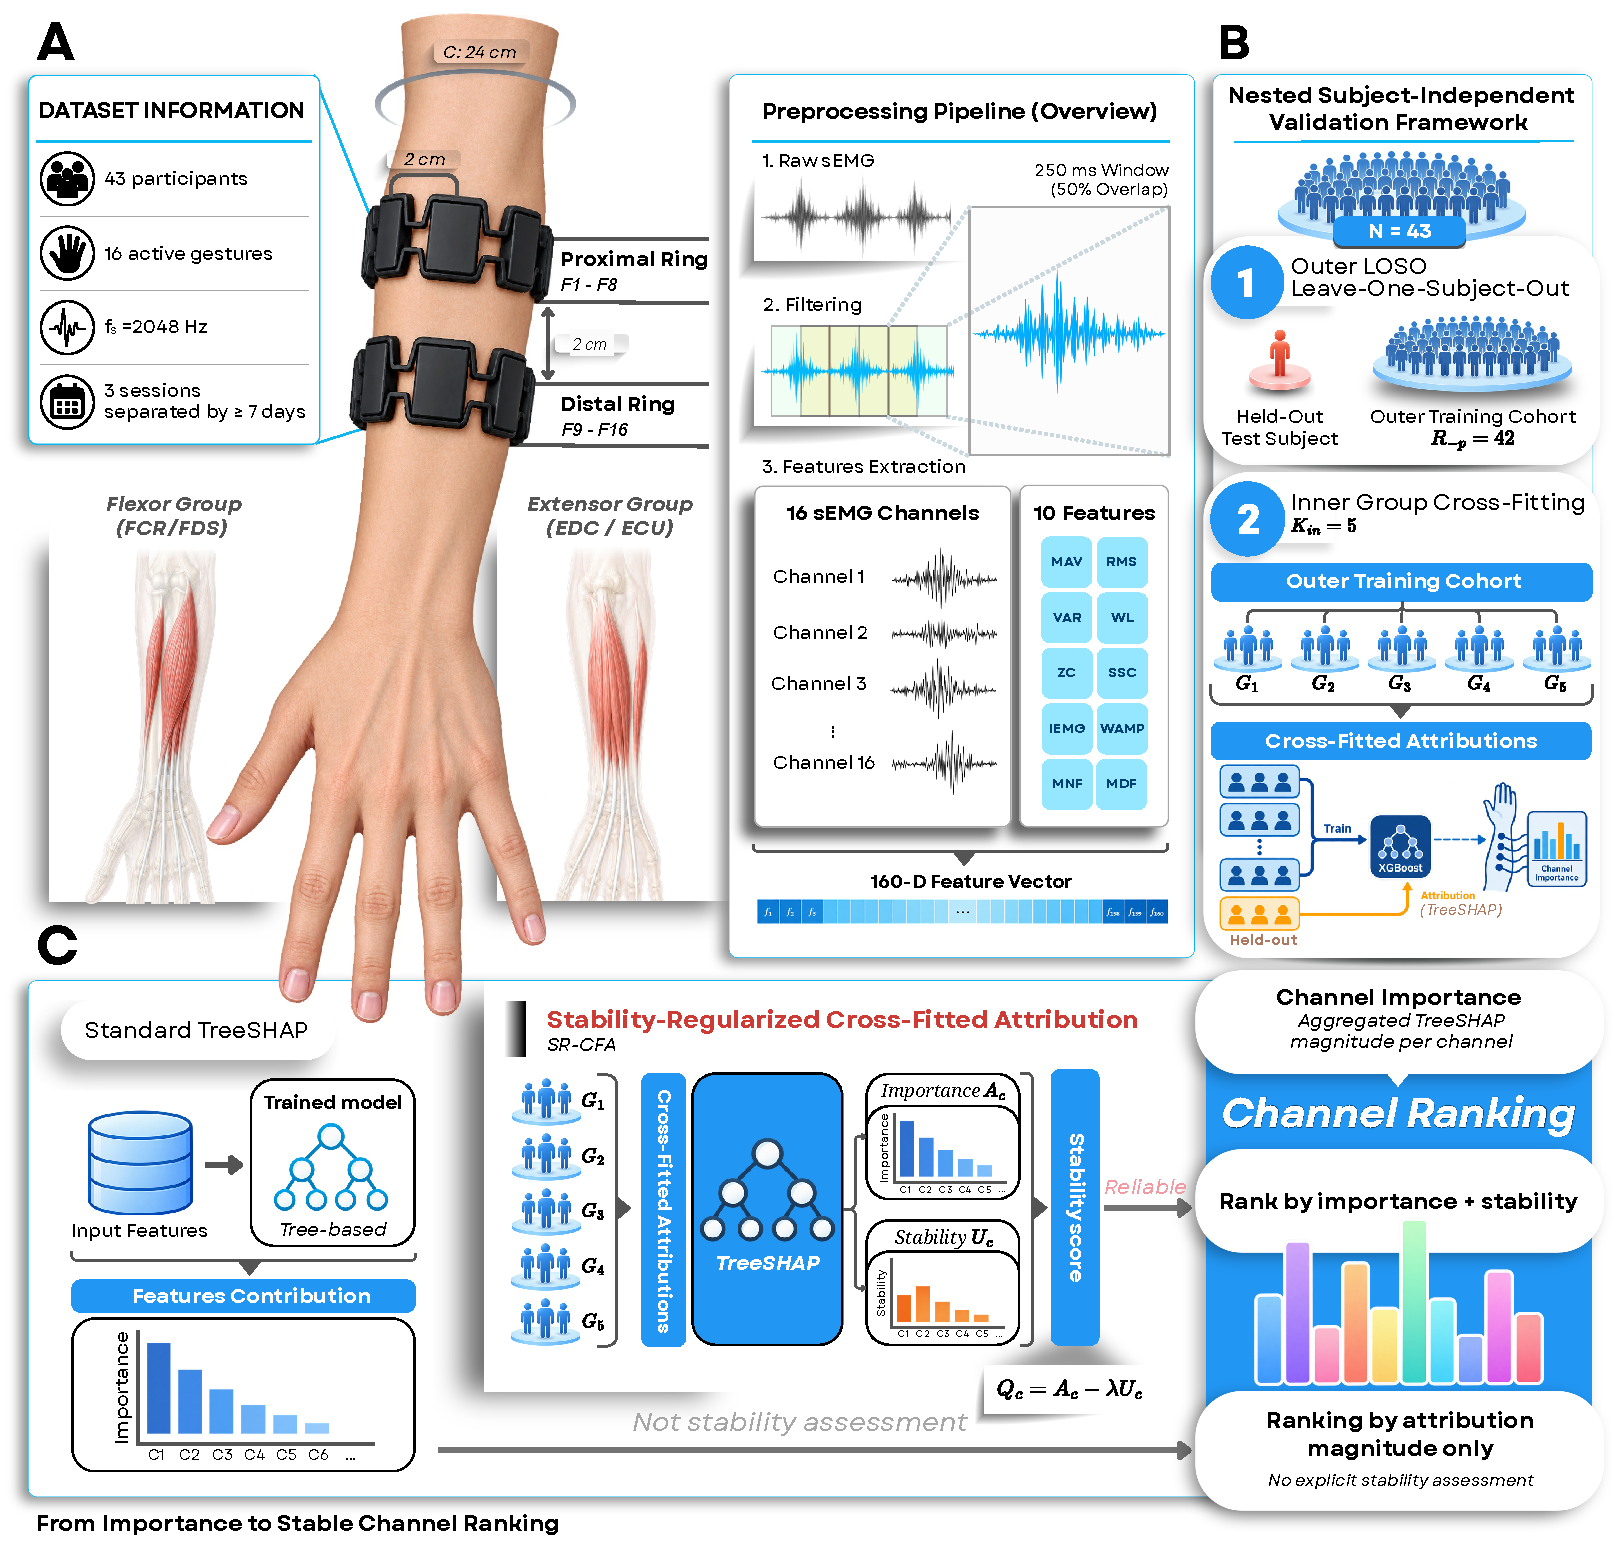
\includegraphics[width=\textwidth]{figures/fig1_overview.pdf}
\caption{Study overview. (A) GRABMyo data and preprocessing: two circumferential rings of eight monopolar electrodes 2~cm apart on the forearm (proximal ring F1--F8, distal ring F9--F16), 250~ms analysis windows with 50\% overlap and ten features per channel (160 features per window). Electrode housings are drawn schematically, and the muscle drawings show general forearm anatomy only; electrodes were not registered to individual muscles. (B) Subject-independent validation: each participant is held out in turn (outer leave-one-subject-out split), and attributions are computed by cross-fitting over five participant-disjoint groups of the remaining participants. (C) The two electrode rankings compared in this study: cross-fitted attribution magnitude alone ($\lambda = 0$) and the stability-regularised score $Q_c = A_c - \lambda U_c$ (SR-CFA). The panel shows how the rankings are formed, not which performed better; the stability penalty produced no statistically detectable improvement (section~\ref{sec:res_attribution}).}
\label{fig:overview}
\end{figure}

\section{Methods}
\label{sec:methods}

\subsection[Datasets and signal processing]{Datasets and signal processing}
\label{sec:datasets}

The primary analysis used GRABMyo v1.1.0 \citep{pradhan2022multiday,jiang2024grabmyo}, distributed through PhysioNet \citep{goldberger2000physionet}, comprising recordings from \GRABMyoParticipants\ able-bodied participants collected over \GRABMyoSessions\ sessions on different days. Participants were \GRABMyoMale\ male and \GRABMyoFemale\ female (age \GRABMyoAgeMean\ $\pm$ \GRABMyoAgeSD\ years). Signals were recorded with an EMGUSB2+ amplifier (OT Bioelettronica) at 2048~Hz; in each session, \chg{each gesture was performed in seven trials of 5~s.} Sixteen monopolar electrodes were positioned in two circumferential rings of eight electrodes around the forearm (F1--F8 and F9--F16), separated longitudinally by 2~cm, with electrode $j$ of one ring aligned with electrode $j+8$ of the other. Mean forearm circumference at the ring position was \GRABMyoCircMean\ $\pm$ \GRABMyoCircSD~cm, giving about \GRABMyoArcSpacing~cm between neighbouring electrodes in a ring. Participants performed 16 active hand and wrist gestures together with rest; the primary recognition task considered the 16 active gestures only, for which \chg{the chance-level} Macro-F1 is about 0.063. All \GRABMyoFilesVerified\ distributed files matched the dataset's published SHA-256 checksums, and all \GRABMyoRecords\ records were analysed.

Terminology is used as follows. An \emph{electrode} is a physical recording site and a \emph{channel} is the signal it provides to the classifier; in the monopolar analyses each electrode yields one channel, so selecting electrodes and selecting channels are the same operation. The \emph{montage} is the spatial arrangement of the electrodes and the \emph{array} is the complete set. A \emph{bipolar pair} is the difference between two electrodes, derived from the monopolar recordings in one exploratory analysis. The subset size $k$ always counts the selection unit of the analysis in question.

NinaPro DB5 \citep{pizzolato2017comparison} was analysed separately as an exploratory replication dataset and was never pooled with GRABMyo. It provides \DBFiveSubjects\ able-bodied \chg{participants} (\DBFiveMale\ male, \DBFiveFemale\ female; age \DBFiveAgeMean\ $\pm$ \DBFiveAgeSD\ years) recorded with two Myo armbands (16 channels, 200~Hz). We used exercise~1 (12 finger movements, 6 repetitions each), segmented with the refined movement and repetition labels supplied with the dataset. \chg{DB5 signals are stored as 8-bit integer codes rather than in physical units,} and its channel numbers have no anatomical correspondence with those of GRABMyo, so only the behaviour of the procedure is compared across datasets.

\paragraph{Ethics statement} This study is a secondary analysis of previously published, de-identified datasets and involved no new participant recruitment or data collection. The original data collections were conducted in accordance with the Declaration of Helsinki and approved by the Office of Research Ethics of the University of Waterloo (ORE\#~31346; GRABMyo) and the Ethics Commission of the Canton of Valais, Switzerland (NinaPro DB5); informed-consent procedures are described in the dataset publications \citep{pradhan2022multiday,pizzolato2017comparison}. [AUTHOR INPUT REQUIRED: state whether an institutional review board determination or exemption was obtained for the present secondary analysis.]

\paragraph{Sex as a reported variable} Sex was taken as reported by the source datasets. Sex-stratified analyses were not prespecified, and the study was not designed to estimate sex differences in recognition performance or electrode ranking; no sex-specific inference is made.

GRABMyo signals were band-pass filtered between 20 and 450~Hz using a fourth-order zero-phase Butterworth filter and notch filtered at 50~Hz ($Q = 30$), the mains frequency identified from the spectra (mean band-power ratio 10.35 at 50~Hz and 0.62 at 60~Hz). Because the filters are zero-phase, the processing is non-causal and suitable only for offline evaluation. Signals were segmented into 250-ms windows with 50\% overlap, without allowing windows to cross trial boundaries. Ten conventional time- and frequency-domain features were extracted from each electrode: mean absolute value, root mean square, variance, waveform length, zero crossings (ZC), slope sign changes (SSC), integrated EMG, Willison amplitude (WAMP), mean frequency and median frequency. The resulting representation contained 160 features per window (\GRABMyoWindows\ windows in total, \GRABMyoActiveWindows\ from active gestures). \chg{The same signal-processing parameters were used in all GRABMyo analyses unless stated otherwise.} The amplitude threshold of the ZC, SSC and WAMP features was set by one rule for every representation: 1.15 times the median absolute first difference of the signal, rounded to one significant figure. For GRABMyo it was computed once, from 54 unfiltered recordings of 6 participants, giving $10^{-2}$~mV; it was therefore not estimated within each outer fold. A leave-one-out check gave the same value in every fold (supplementary methods~S2), so fold-wise estimation would have produced identical features. DB5 was band-pass filtered at 10--95~Hz without a notch filter, with 250~ms windows (50 samples) and a threshold of 7 quantisation steps from the same rule; the leave-one-out recomputation gave the same threshold in every DB5 fold.

\subsection[Subject-independent electrode ranking and model evaluation]{Subject-independent electrode ranking and model evaluation}
\label{sec:ranking}

All primary evaluations followed an outer leave-one-subject-out (LOSO) design (figure~\ref{fig:workflow}). For each held-out participant $p$, all preprocessing statistics, model fitting and electrode ranking were derived exclusively from the remaining participants $R_{-p}$. The held-out participant contributed only to the final performance estimate.

\begin{figure}[t]
\centering
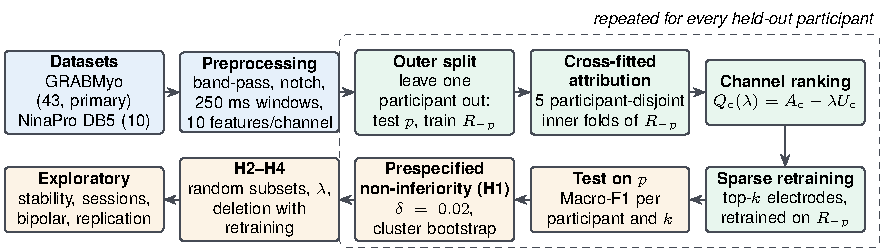
\includegraphics[width=\textwidth]{figures/fig2_workflow.pdf}
\caption{Study workflow. For each held-out participant $p$, feature standardisation, model fitting and electrode ranking use only the remaining participants $R_{-p}$. Attributions are computed on participant-disjoint inner folds of $R_{-p}$, and models restricted to the top-ranked $k$ electrodes are retrained on $R_{-p}$ and tested on $p$. The same workflow was applied separately to each dataset.}
\label{fig:workflow}
\end{figure}

XGBoost was used as the primary classifier for the electrode-selection experiments because the analysis required repeated model retraining across participants, electrode counts and selection strategies. It was designated in the analysis plan on these computational grounds; the plan was written before the full-cohort classifier comparison had finished, although results from an earlier, superseded run on 15 participants were available. XGBoost used 300 trees, depth 6, learning rate 0.1, row and column subsampling of 0.8, histogram-based tree construction and a multiclass softmax objective, and was trained on all \FoldTrainingWindows\ training windows of each fold. Support vector machine and random forest models were additionally evaluated using the complete array to provide classifier-level context: a support vector machine with a radial basis function kernel ($C = 1$, kernel width set from the feature variance), trained on a stratified sample of 40,000 windows, and a random forest (200 trees, minimum leaf size 2) trained on 200,000 windows. These sample sizes were \chg{constrained} by computational cost and chosen \chg{using} two folds (supplementary methods~S1). Halving the support vector machine's training sample on one fold lowered Macro-F1 from \SVMCalibFortyK\ to \SVMCalibTwentyK, so its \chg{reported performance is probably} a lower bound. Classifier hyperparameters were fixed for the reported runs. Because this \chg{budget calibration used the outcomes of two test folds, model development} was not fully isolated from the evaluation cohort.

Electrode importance was estimated within each outer training set using $K = 5$ participant-disjoint inner folds. For each inner fold $j$, an XGBoost model was trained on the remaining inner participants and TreeSHAP values were evaluated on the participants excluded from that model. Each inner model used a random sample of at most 200,000 windows standardised with inner-training statistics only, and exact tree-path-dependent TreeSHAP attributions on raw model margins \citep{lundberg2020local} were computed for up to 20,000 windows sampled at random from the inner-held-out participants. Because participants contribute similar numbers of windows (median \TestWindowsPerParticipant), each participant carries \chg{approximately equal weight in the attribution.} In every fold we verified that no inner-held-out participant contributed to the corresponding inner training set. Absolute attributions were averaged over the $G = 16$ classes and the $F = 10$ features belonging to each electrode,
\begin{equation}
\Phi_{i,c} = \frac{1}{G F}\sum_{g=1}^{G}\sum_{f=1}^{F} \lvert \phi_{i,g,c,f} \rvert,
\end{equation}
then averaged over windows and normalised across electrodes to give $I_{j,c}$. The resulting cross-fitted attribution magnitude $A_c = \operatorname{median}_j I_{j,c}$ represented the typical importance of electrode $c$, whereas $U_c = \operatorname{median}_j \lvert I_{j,c} - A_c \rvert$ quantified its variation across inner folds\chg{; $U_c$ is large when the importance of an electrode depends on which participants were used to estimate it}. Electrodes were ranked according to
\begin{equation}
Q_c(\lambda) = A_c - \lambda\, U_c, \qquad \lambda \in \{0, 0.25, 0.5, 1\},
\label{eq:srcfa}
\end{equation}
where $\lambda = 0$ corresponds to cross-fitted attribution magnitude alone and positive values introduce a penalty for unstable attribution (the stability-regularised cross-fitted attribution score, SR-CFA). Ties were broken by the lower channel number. The plan did not specify a criterion for choosing $\lambda$, so all four values are reported.

For each outer fold, each $\lambda$ and each retained electrode count $k \in \{1, \ldots, 16\}$, the classifier was retrained from scratch using only the top-$k$ electrodes and evaluated on the held-out participant. All models of this electrode-count performance curve used the same fixed, stratified sample of 200,000 training windows of the fold. This separation between ranking and final evaluation ensured that neither electrode selection nor model training used information from the participant on whom performance was measured. \chg{Three training configurations were therefore used, and results are compared only within a configuration: the full-array classifier comparison (all training windows of each fold), the performance curve used for H1 and H3 (the 200,000-window sample above) and a lighter comparison model used for H2, H4 and the exploratory selection methods (described below). The 16-electrode results of these configurations differ slightly for this reason.}

\subsection[Hypothesis testing and statistical analysis]{Hypothesis testing and statistical analysis}
\label{sec:statistics}

The primary endpoint was participant-level Macro-F1 across the 16 active gestures\chg{, the unweighted mean of the per-gesture F1 scores, so that every gesture counts equally}; accuracy and balanced accuracy were also recorded. For each reduced configuration, performance was compared with the 16-electrode model of the same curve, trained using the same outer-fold data. The paired difference for participant $p$ and subset size $k$ was defined as
\begin{equation}
\Delta_{p,k} = \mathrm{F1}_{p,k} - \mathrm{F1}_{p,16}.
\end{equation}
A subset was considered non-inferior (H1) when $L_k$, the lower bound of the 95\% participant-cluster-bootstrap confidence interval for the mean paired difference $\bar\Delta_k$, exceeded the prespecified margin $-\delta$ with $\delta = 0.02$ Macro-F1. The smallest subset satisfying this criterion defined the minimum acceptable electrode count, $k^* = \min\{k < 16 : L_k > -\delta\}$, recorded as `none' if no $k$ qualifies. As required by the plan, the family of 15 tests was also \chg{Holm-corrected}, using one-sided cluster-bootstrap $p$-values for $H_0\colon \bar\Delta_k \le -\delta$ at $\alpha = 0.025$ \chg{(the proportion of bootstrap means at or below $-\delta$)}. The margin is an absolute difference in Macro-F1 on a 0--1 scale, fixed before the curve was computed as the largest loss we would accept in exchange for fewer electrodes. Relative to the \chg{mean Macro-F1 of the 16-electrode curve reference,} it corresponds to about \MarginPctOfRef\% of performance and about \MarginPctAboveChance\% of the distance above chance (1/16). It is an engineering tolerance and has not been validated against clinical outcomes or user performance. Because $k^*$ depends on $\delta$, sensitivity analyses were additionally performed at the prespecified margins of 0.01 and 0.03. Non-inferiority within this tolerance does not imply equivalence.

To determine whether the attribution ranking conveyed useful information beyond chance (H2), attribution-selected subsets were compared with random subsets of identical size at $k = 4$, 6, 8 and 12. Additional exploratory comparisons included permutation importance, mutual information and geometric farthest-point selection. Every ranking was computed on the training participants only:
\begin{itemize}
\item SR-CFA ($\lambda = 0.5$) and cross-fitted SHAP ($\lambda = 0$);
\item permutation importance: a model was fitted on 20,000 training windows and each of the 160 features was permuted in 8,000 further windows (3 repeats, Macro-F1 scoring); an electrode's score is the mean over its 10 features;
\item mutual information between each feature and the gesture label on the same 20,000 windows, averaged over the electrode's 10 features;
\item geometric selection: farthest-point sampling on the $2 \times 8$ montage (arc distance around a 24~cm circumference, 2~cm between rings, starting from F1, ties to the lower index), which uses no data;
\item random subsets: 100 independent random subsets per participant at each $k$, and 500 at $k = 12$, as the plan required at $k^*$ (seed fixed per participant).
\end{itemize}
Evaluating hundreds of random subsets per participant required a lighter comparison model (XGBoost with 50 trees, trained on a stratified sample of 150,000 windows), applied identically to every method; its absolute scores are lower than those of the performance curve and are compared only with each other. The H2 test family contrasts each of the two attribution rankings with the participant's mean over its random subsets at the four subset sizes (8 tests, Holm-corrected); comparisons with permutation importance, mutual information and geometric selection are exploratory and uncorrected. We also report the percentile of the SR-CFA subset within each participant's random subsets\chg{, that is, the proportion of that participant's random subsets that scored lower than the SR-CFA subset}. Below, `SR-CFA' refers to $\lambda = 0.5$ and `cross-fitted SHAP' to $\lambda = 0$.

Stability regularisation (H3) was assessed by comparing each $\lambda > 0$ with $\lambda = 0$ on the performance curve at $k = 4$, 6, 8 and 12 (Holm over 12 tests). Attribution faithfulness (H4) was assessed through deletion with retraining \citep{samek2017evaluating,hooker2019benchmark}: performance was measured after preferentially removing highly ranked (Remove-Top), randomly selected (Remove-Random) or weakly ranked (Remove-Bottom) electrodes. For $n \in \{2, 4, \ldots, 14\}$ electrodes retained, the comparison model was retrained after removing the $16 - n$ highest- or lowest-ranked electrodes; Remove-Random used the random subsets above and is available for $n \in \{4, 6, 8, 12\}$. A faithful ranking gives Remove-Top $<$ Remove-Random $<$ Remove-Bottom. Paired contrasts were Holm-corrected within H4 (15 tests).

The participant, rather than the individual signal window, was treated as the statistical unit throughout ($n = 43$ for GRABMyo, 10 for DB5); no participant was excluded. Confidence intervals (CI) were obtained as 95\% percentile intervals from 10,000 participant-level cluster-bootstrap resamples (seed 20260728)\chg{, in which whole participants, with all their windows, were resampled with replacement}. Because LOSO training sets overlap, these intervals quantify variation in the observed out-of-fold participant scores and do not fully propagate uncertainty from retraining on a new cohort. Paired comparisons used the Wilcoxon signed-rank test with the matched-pairs rank-biserial correlation $r_{rb}$ as the effect size, and Holm correction was applied within each hypothesis family (H1--H4). \chg{The plan named H1--H4 as confirmatory hypotheses, but} the detailed H2--H4 families (subset sizes and rankings compared) were specified after the underlying results were available; these are therefore reported as secondary tests, distinct from the primary H1 decision rule. Effect sizes and confidence intervals for every H2--H4 contrast are reported in table~\ref{tab:h2} and supplementary tables S5 and S6. \chg{A non-significant difference was interpreted as an absence of statistically detectable evidence, not as evidence of equivalence; no equivalence tests were performed.}

\subsection[Exploratory and sensitivity analyses]{Exploratory and sensitivity analyses}
\label{sec:exploratory}

Exploratory analyses examined the stability of electrode rankings across participants, replication of the reduction procedure on NinaPro DB5, cross-session generalisation within GRABMyo, and bipolar re-referencing of the original monopolar recordings. These analyses were interpreted separately from the primary non-inferiority test. A fixed-layout consistency check, in which one 12-electrode layout was derived on \chg{one half of the participants and tested on the other half, in both directions,} is described in supplementary methods~S4; \chg{because the electrode count was chosen after the full-cohort curve had been inspected, it} is not an independent validation of the electrode count.

\paragraph{Ranking stability} We compared rankings derived from single participants' attributions (all 903 pairs), from the five inner folds and from the 43 outer folds, using Spearman's $\rho$, Kendall's $\tau$ and the Jaccard index of the top-$k$ sets. A participant's attribution profile is the mean of their normalised attribution over the outer folds in which they were held out of an inner model. Outer folds share about 98\% of their training participants, so their agreement is not an independent estimate of between-person stability.

\paragraph{Replication} The LOSO baseline, cross-fitted ranking ($K = 5$) and performance curve were repeated on DB5, with its full array as reference ($k = 16$), using all training windows and the same bootstrap, margins and $k^*$ rule. Holm-corrected results are also reported. No setting was tuned on DB5. \chg{As a post-hoc diagnostic of Monte Carlo variation, the DB5 and bipolar bootstraps were repeated with 200 different random seeds, and the number of reruns giving a non-inferior decision is reported; this describes the stability of the decision, not the probability that it is correct.}

\paragraph{Cross-session} \chg{In one design (CS1), XGBoost was trained on session~1 of $R_{-p}$ and tested on each session of $p$; in the other (CS2), it was trained on sessions 1 and 2 and tested on session~3.} These comparisons use the full array and do not test a reduced layout under session transfer. The second condition also has about twice the training data, so it confounds session diversity with data quantity.

\paragraph{Bipolar re-referencing} To use a bipolar pair as the selection unit, we formed $B_j = F_j - F_{j+8}$ ($j = 1, \ldots, 8$) from the monopolar recordings, re-extracted features with the threshold given by the same rule ($4 \times 10^{-3}$~mV; the bipolar signal is about half the monopolar amplitude), and repeated the analysis with the $k = 8$ model as reference. These are derived pairs, not physical bipolar electrodes.

\paragraph{Participant-level aggregation (post hoc)} \chg{In the primary score, $A_c$ and $U_c$ are computed over five inner-fold attribution vectors, each of which pools several participants, so $U_c$ reflects variation between groups of participants rather than between individuals. A post-hoc extension therefore computed the median and the unscaled median absolute deviation over the individual attribution vectors of all outer-training participants, one vector per participant.} The same score and all four penalties were evaluated at every subset size under the original performance-curve model and training budget, and no penalty was selected from outer-test performance. Exact duplicate electrode sets reused the same fitted evaluation. Comparisons against the original aggregation were paired by participant, and the family of all reduced-size comparisons across penalties received Holm correction. Person vectors share inner models, so their dispersion measures heterogeneity rather than a standard error.

Departures from the original statistical analysis plan are documented in supplementary methods~S1. These included post-hoc specification of the detailed H2--H4 test families, application of the plan's Holm correction for H1 after the primary analysis, selection of computational training budgets using two folds, and addition of fixed-layout, feature-redundancy and participant-level attribution analyses; two exploratory analyses listed in the plan were not run. None altered the prespecified non-inferiority margin, statistical unit, bootstrap procedure or definition of the minimum acceptable electrode count.

\section{Results}
\label{sec:results}

\subsection[Subject-independent performance and electrode reduction]{Subject-independent performance and electrode reduction}
\label{sec:res_reduction}

With all 16 electrodes, XGBoost achieved a mean Macro-F1 of \FullXGB\ (95\% CI \FullXGBLCB--\FullXGBUCB) across the 43 held-out participants. The corresponding values were \FullSVM\ (95\% CI \FullSVMLCB--\FullSVMUCB) for the support vector machine and \FullRF\ (95\% CI \FullRFLCB--\FullRFUCB) for the random forest (figure~\ref{fig:full}; supplementary table~S1). No statistically detectable difference was observed between XGBoost and the support vector machine (paired difference $\XGBvsSVMDiff$, 95\% CI $\XGBvsSVMLCB$ to $\XGBvsSVMUCB$, $p_{\mathrm{Holm}} \XGBvsSVMP$, $r_{rb} = \XGBvsSVMR$), whereas both models outperformed the random forest ($p_{\mathrm{Holm}} \XGBvsRFP$ and $\SVMvsRFP$; $r_{rb} = \XGBvsRFR$ and $\SVMvsRFR$). Between-participant variability was substantially larger than the difference between the two higher-performing classifiers: XGBoost ranged from \FullXGBMin\ to \FullXGBMax\ across participants. Per-gesture F1, reconstructed from the saved full-array predictions, is reported in supplementary table~S2.

\begin{figure}[t]
\centering
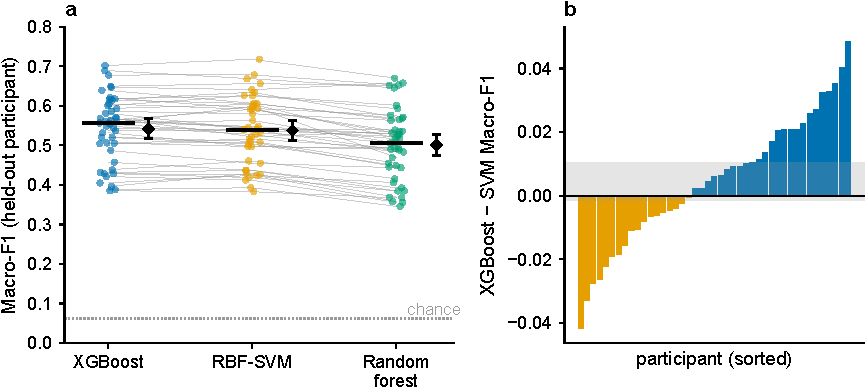
\includegraphics[width=\textwidth]{figures/fig3_full_channel.pdf}
\caption{Full-array leave-one-subject-out performance on GRABMyo (43 participants). (a) Macro-F1 of three classifiers; each point is one held-out participant, grey lines join the same participant, black bars mark medians and diamonds mark means with 95\% cluster-bootstrap confidence intervals. The support vector machine and random forest were trained on samples of 40,000 and 200,000 windows. (b) Paired XGBoost minus support vector machine difference per participant, sorted; the grey band is the 95\% confidence interval of the mean difference.}
\label{fig:full}
\end{figure}

Recognition performance decreased progressively as electrodes were removed (figure~\ref{fig:curve}, table~\ref{tab:sparse_ni}). \chg{The 16-electrode reference of the curve scored \CurveKSixteen, slightly below the full-array result, consistent with the smaller training sample (200,000 windows) shared by all curve models.} Under the prespecified margin of 0.02 Macro-F1, the smallest non-inferior configuration contained $k^* = \KStar$ electrodes. Its mean difference from the corresponding 16-electrode reference was $\DeltaKTwelve$ (95\% CI $\DeltaKTwelveLCB$ to $\DeltaKTwelveUCB$), whereas \chg{the lower confidence bound for 11 electrodes ($\DeltaKElevenLCB$) fell below the margin.} All configurations containing 12--15 electrodes satisfied the criterion, and the minimum acceptable count remained \KStarHolm\ after Holm correction ($k = 12$: $p_{\mathrm{Holm}} \HolmPKTwelve$). As expected, the \chg{minimum count depended on the margin}: the minimum was \KStarMarginPtOne\ electrodes at $\delta = 0.01$ and \KStarMarginPtThree\ at $\delta = 0.03$, again unchanged by Holm correction (supplementary table~S3).

\begin{table*}[t]
\centering
\small
\caption{Electrode-count performance curve and primary non-inferiority decision on GRABMyo (cross-fitted ranking, $\lambda = 0$; 43 participants; every $k$ retrained from scratch on the same 200,000 training windows of each fold). $\Delta_k$: mean paired difference from the $k = 16$ model of the same curve, with 95\% participant cluster-bootstrap confidence interval (CI). Non-inferior: lower bound above $-\delta$ with the primary margin $\delta = 0.02$; Holm: the same decision after Holm correction over the 15 subset sizes. The smallest non-inferior subset ($k^*$) is in bold; the rule below it marks the boundary. Decisions at the sensitivity margins $\delta = 0.01$ and 0.03 are given in supplementary table S3.}
\label{tab:sparse_ni}
\setlength{\tabcolsep}{4pt}
\begin{adjustbox}{max width=\textwidth}
\begin{tabular}{rccccc}
\toprule
$k$ & Macro-F1 (mean $\pm$ SD) & $\Delta_k$ & 95\% CI & Non-inferior & Non-inferior (Holm) \\
\midrule
16 & 0.541 $\pm$ 0.084 & reference &  &  &  \\
15 & 0.538 $\pm$ 0.083 & $-$0.0036 & $-$0.0056 to $-$0.0017 & yes & yes \\
14 & 0.535 $\pm$ 0.083 & $-$0.0060 & $-$0.0081 to $-$0.0039 & yes & yes \\
13 & 0.530 $\pm$ 0.083 & $-$0.0109 & $-$0.0133 to $-$0.0085 & yes & yes \\
\textbf{12} & \textbf{0.528 $\pm$ 0.084} & \textbf{$-$0.0133} & \textbf{$-$0.0160 to $-$0.0106} & \textbf{yes} & \textbf{yes} \\
\midrule 11 & 0.521 $\pm$ 0.084 & $-$0.0204 & $-$0.0246 to $-$0.0162 & no & no \\
10 & 0.515 $\pm$ 0.083 & $-$0.0259 & $-$0.0311 to $-$0.0205 & no & no \\
9 & 0.510 $\pm$ 0.086 & $-$0.0318 & $-$0.0387 to $-$0.0246 & no & no \\
8 & 0.505 $\pm$ 0.085 & $-$0.0366 & $-$0.0440 to $-$0.0289 & no & no \\
7 & 0.500 $\pm$ 0.085 & $-$0.0413 & $-$0.0489 to $-$0.0333 & no & no \\
6 & 0.480 $\pm$ 0.084 & $-$0.0610 & $-$0.0713 to $-$0.0507 & no & no \\
5 & 0.428 $\pm$ 0.075 & $-$0.1133 & $-$0.1277 to $-$0.0993 & no & no \\
4 & 0.397 $\pm$ 0.071 & $-$0.1444 & $-$0.1590 to $-$0.1306 & no & no \\
3 & 0.340 $\pm$ 0.057 & $-$0.2015 & $-$0.2212 to $-$0.1822 & no & no \\
2 & 0.299 $\pm$ 0.057 & $-$0.2420 & $-$0.2603 to $-$0.2230 & no & no \\
1 & 0.181 $\pm$ 0.040 & $-$0.3603 & $-$0.3832 to $-$0.3369 & no & no \\
\bottomrule
\end{tabular}
\end{adjustbox}
\end{table*}


\begin{figure}[t]
\centering
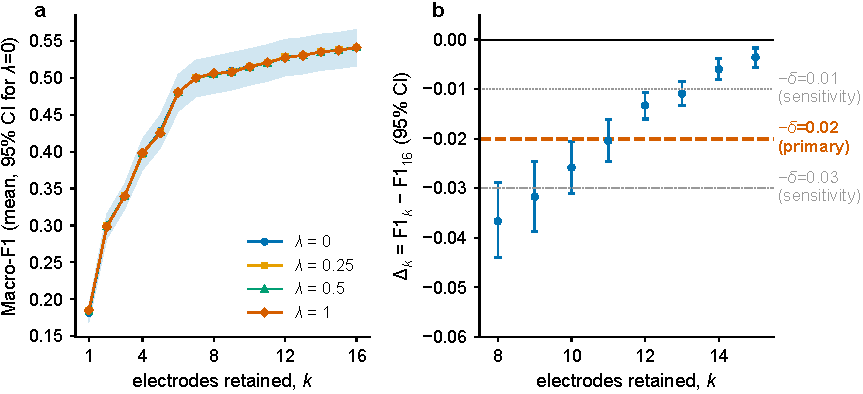
\includegraphics[width=\textwidth]{figures/fig4_sparse_curve.pdf}
\caption{Electrode-count performance curve on GRABMyo (43 participants). (a) Mean Macro-F1 of models retrained on the top-$k$ electrodes of each fold's cross-fitted ranking, for the four values of the stability weight $\lambda$ (the curves overlap); the band is the 95\% cluster-bootstrap confidence interval for $\lambda = 0$. (b) Paired difference to the $k = 16$ model with 95\% confidence interval. The thick dashed line marks the primary margin ($-\delta$, $\delta = 0.02$); the thin dotted and dash-dotted grey lines mark the sensitivity margins (0.01 and 0.03).}
\label{fig:curve}
\end{figure}

Thus, a \KStarReductionPct\% reduction in electrode count was supported within the prespecified engineering tolerance, whereas larger reductions were not. Halving the array to eight electrodes gave a mean difference of $\DeltaKEight$ (95\% CI $\DeltaKEightLCB$ to $\DeltaKEightUCB$), and every reduced configuration had a numerically lower \chg{mean} Macro-F1 than the complete array. Because the ranking was recomputed within every outer fold, this result characterises the electrode count reached by the selection procedure rather than one fixed layout; in practice the procedure excluded the same electrodes (\DroppedFourSet) at $k = 12$ in \DroppedFourFolds\ of 43 folds. \chg{When one 12-electrode layout was instead frozen on half of the participants and tested on the other half, the mean loss was $\FixedDiff$ and $\FixedSwapDiff$ in the two directions; the criterion was met in the first direction and missed narrowly in the second (lower bound $\FixedSwapLCBSix$; supplementary methods~S4).}

\subsection[Evaluation of attribution-guided electrode selection]{Evaluation of attribution-guided electrode selection}
\label{sec:res_attribution}

Both attribution rankings outperformed the mean random-subset baseline at all four tested subset sizes (table~\ref{tab:h2}; 8 tests, Holm-corrected). \chg{The advantage of SR-CFA was largest at six electrodes} ($\HTwoKSixDiff$ Macro-F1, 95\% CI $\HTwoKSixLCB$ to $\HTwoKSixUCB$, $p_{\mathrm{Holm}} \HTwoKSixP$, $r_{rb} = \HTwoKSixR$) \chg{and eight electrodes ($\HTwoKEightDiff$). It was smaller at 12 electrodes ($\HTwoKTwelveDiff$, $p_{\mathrm{Holm}} \HTwoKTwelveP$), where the retained array is close to the full array, and at four electrodes ($\HTwoKFourDiff$).} Cross-fitted SHAP and SR-CFA gave identical results at $k = 6$ and 12 and similar results at $k = 4$ and 8 (table~\ref{tab:h2})\chg{, because the two rankings selected the same subsets for \HTwoSameKSix\ and \HTwoSameKTwelve\ of 43 participants at $k = 6$ and 12 and for \HTwoSameKFour\ and \HTwoSameKEight\ at $k = 4$ and 8}. \chg{Outperforming the mean of the random subsets did not mean outperforming most of them for each participant}: the median percentile of the SR-CFA subset within each participant's random-subset distribution was \PctKFour, \PctKSix, \PctKEight\ and \PctKTwelve\ at $k = 4$, 6, 8 and 12, and it reached the 95th percentile for \PctKAboveNinetyFiveSix\ of 43 participants at $k = 6$ and \PctKAboveNinetyFiveTwelve\ at $k = 12$ (figure~\ref{fig:baselines}(b)).

\begin{table*}[t]
\centering
\small
\caption{\chg{H2: attribution-ranked subsets versus the mean of random subsets of the same size (GRABMyo, 43 participants; secondary family of 8 tests, Holm-corrected; the detailed test family was specified after the underlying results were available). All subsets were evaluated with one comparison model (XGBoost, 50 trees, 150,000 training windows per fold), so absolute values are lower than in table~\ref{tab:sparse_ni}. Random: participant's mean over 100 random subsets (500 at $k = 12$). Difference: mean paired difference (attribution minus random) with 95\% participant cluster-bootstrap confidence interval (CI). Higher/lower: participants for whom the attribution subset scored above/below their random mean. $p_{\mathrm{Holm}}$: Wilcoxon signed-rank, Holm-corrected; $r_{rb}$: matched-pairs rank-biserial correlation.}}
\label{tab:h2}
\setlength{\tabcolsep}{4pt}
\begin{adjustbox}{max width=\textwidth}
\begin{tabular}{rlccccccc}
\toprule
$k$ & Ranking & Attribution & Random & Difference & 95\% CI & Higher/lower & $p_{\mathrm{Holm}}$ & $r_{rb}$ \\
\midrule
4 & Cross-fitted SHAP ($\lambda = 0$) & 0.382 & 0.366 & +0.0163 & +0.0060 to +0.0267 & 29/14 & 0.007 & +0.47 \\
 & SR-CFA ($\lambda = 0.5$) & 0.383 & 0.366 & +0.0172 & +0.0071 to +0.0274 & 30/13 & 0.007 & +0.50 \\
\midrule 6 & Cross-fitted SHAP ($\lambda = 0$) & 0.453 & 0.416 & +0.0370 & +0.0286 to +0.0452 & 37/6 & $<$0.001 & +0.92 \\
 & SR-CFA ($\lambda = 0.5$) & 0.453 & 0.416 & +0.0370 & +0.0286 to +0.0452 & 37/6 & $<$0.001 & +0.92 \\
\midrule 8 & Cross-fitted SHAP ($\lambda = 0$) & 0.468 & 0.445 & +0.0230 & +0.0161 to +0.0298 & 36/7 & $<$0.001 & +0.82 \\
 & SR-CFA ($\lambda = 0.5$) & 0.469 & 0.445 & +0.0243 & +0.0176 to +0.0308 & 37/6 & $<$0.001 & +0.86 \\
\midrule 12 & Cross-fitted SHAP ($\lambda = 0$) & 0.485 & 0.478 & +0.0074 & +0.0046 to +0.0103 & 35/8 & $<$0.001 & +0.71 \\
 & SR-CFA ($\lambda = 0.5$) & 0.485 & 0.478 & +0.0074 & +0.0046 to +0.0103 & 35/8 & $<$0.001 & +0.71 \\
\bottomrule
\end{tabular}
\end{adjustbox}
\end{table*}


In exploratory, uncorrected contrasts (figure~\ref{fig:baselines}(a); supplementary table~S4), no statistically detectable difference between SR-CFA and permutation importance was observed at $k = 4$, 8 or 12 (for example, $k = 8$: $\VSPermKEightDiff$, $p \VSPermKEightP$); at $k = 6$, SR-CFA was higher by $\VSPermKSixDiff$ ($p \VSPermKSixP$). Likewise, no statistically detectable difference between SR-CFA and geometric selection, which spreads electrodes evenly around both rings without using data, was observed at $k = 4$ ($\VSGeomKFourDiff$, $p \VSGeomKFourP$), $k = 8$ ($\VSGeomKEightDiff$, $p \VSGeomKEightP$) or $k = 12$ ($\VSGeomKTwelveDiff$, $p \VSGeomKTwelveP$); at $k = 6$, SR-CFA was higher by $\VSGeomKSixDiff$ ($p \VSGeomKSixP$). Mutual information gave the lowest \chg{mean scores of all methods at every $k \le 8$, below the random-subset mean.}

\begin{figure}[t]
\centering
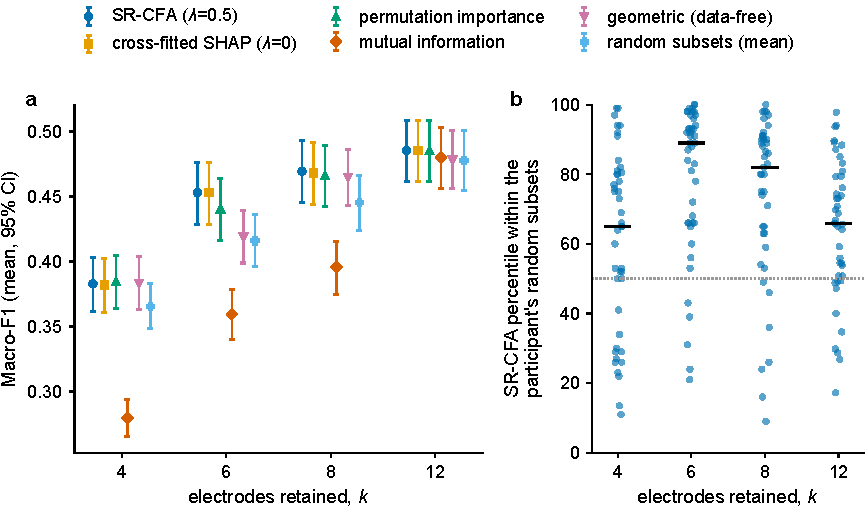
\includegraphics[width=\textwidth]{figures/fig5_selection_baselines.pdf}
\caption{Electrode-selection methods at matched subset size $k$ (GRABMyo, 43 participants; one comparison model shared by all methods). (a) Mean Macro-F1 with 95\% cluster-bootstrap confidence intervals, grouped by method type: attribution rankings (stability-regularised cross-fitted attribution, SR-CFA, and cross-fitted SHAP), model-based rankings (permutation importance and mutual information), data-free geometric selection and the mean over random subsets. (b) Percentile of the SR-CFA subset within each participant's own random subsets (one point per participant; bar = median; 100 random subsets per participant, 500 at $k = 12$).}
\label{fig:baselines}
\end{figure}

Deletion with retraining supported the faithfulness of the ranking (figure~\ref{fig:faithfulness}; supplementary table~S5). Mean Macro-F1 followed the order Remove-Top $<$ Remove-Random $<$ Remove-Bottom at every number of retained electrodes for which all three orders were available, and Remove-Top $<$ Remove-Bottom at every number retained; \FaithNSig\ of the \FaithNTests\ Holm-corrected contrasts were significant. With six electrodes retained, Remove-Top scored \FaithTopKSix, Remove-Random \FaithRandomKSix\ and Remove-Bottom \FaithBottomKSix\ (Remove-Top minus Remove-Random $\FaithTRKSixDiff$, $p_{\mathrm{Holm}} \FaithTRKSixP$; Remove-Random minus Remove-Bottom $\FaithRBKSixDiff$, $p_{\mathrm{Holm}} \FaithRBKSixP$). The separation was largest at intermediate subset sizes and smaller near the extremes, where either very few or nearly all electrodes remained; the Remove-Top versus Remove-Bottom contrast with 14 electrodes retained, where only two electrodes are removed, was not statistically significant ($\FaithTBKFourteenDiff$, $p_{\mathrm{Holm}} \FaithTBKFourteenP$).

\begin{figure}[t]
\centering
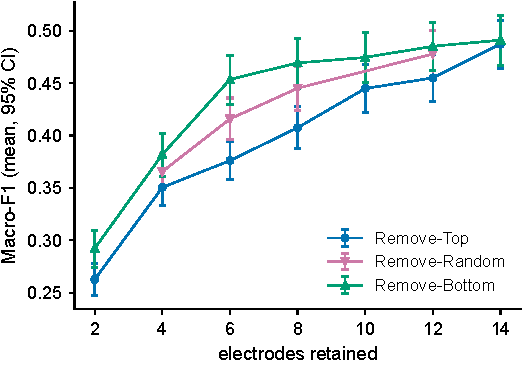
\includegraphics[width=0.62\textwidth]{figures/fig6_faithfulness.pdf}
\caption{Deletion-with-retraining test of attribution faithfulness on GRABMyo (43 participants; mean and 95\% cluster-bootstrap confidence interval). Remove-Top deletes the highest-ranked electrodes, Remove-Bottom the lowest-ranked and Remove-Random a random set; all use the same comparison model and training sample. Remove-Random is shown where random subsets were sampled (4, 6, 8 and 12 electrodes retained).}
\label{fig:faithfulness}
\end{figure}

Stability regularisation did not provide a statistically detectable improvement. Attribution variability across the inner participant groups was small relative to attribution magnitude (median $U_c/A_c$ \UOverAMedian\%, maximum \UOverAMax\%), so positive values of $\lambda$ rarely changed the selected subsets. Relative to $\lambda = 0$, the top-12 set changed in \TopTwelveDiffersLambdaPtTwoFive, \TopTwelveDiffersLambdaPtFive\ and \TopTwelveDiffersLambdaOne\ of 43 folds at $\lambda = 0.25$, 0.5 and 1, and across all four $k$ tested at least \HThreeMinTied\ of 43 participants received the identical subset under both rankings. None of the \HThreeNTests\ contrasts was significant after Holm correction (largest mean difference \HThreeMaxAbsDiff; smallest $p_{\mathrm{Holm}} \HThreeMinP$; supplementary table~S6). The four curves in figure~\ref{fig:curve}(a) differ by at most \LambdaCurveMaxSpread, and $k^*$ was identical under every $\lambda$ and margin; H3 was not supported. A post-hoc participant-level aggregation increased the estimated attribution heterogeneity but did not change $k^*$ under any penalty\chg{; it showed no Holm-corrected difference in performance from fold-level aggregation and no benefit of the penalty within participant-level aggregation} (supplementary methods~S6, table~S7 and figures~S1--S2).

\subsection[Robustness and exploratory analyses]{Robustness and exploratory analyses}
\label{sec:res_exploratory}

Electrode rankings showed substantial agreement across participants, particularly at the upper and lower ends of the ranking (table~\ref{tab:stability}, figure~\ref{fig:attribution}). Rankings computed from individual participants' attributions agreed closely (mean Spearman $\rho$ = \StabSubjRho\ $\pm$ \StabSubjRhoSD\ over \StabSubjPairs\ pairs; mean Jaccard index of the top six \StabSubjJacSix), and rankings from disjoint inner folds agreed at $\rho$ = \StabInnerRho. The same four electrodes (\TopFourSet) formed the top four in \TopFourFolds\ of 43 outer folds and carried \TopFourShare\% of the summed attribution, whereas the eight lowest-ranked electrodes carried \BottomEightShare\%; rank ranges were widest in the middle of the ordering. The outer-fold agreement ($\rho$ = \StabOuterRho) is descriptive only, because those training sets share about 98\% of their participants. \chg{These results indicate} that the subject-independent procedure identified \chg{consistent} spatial preferences, although the data do not support assigning these positions to individual muscles.

\begin{table*}[t]
\centering
\small
\caption{Agreement of electrode rankings on GRABMyo ($\lambda = 0$). Values are mean (SD) over all pairs of rankings in each group. They are descriptive summaries: pairwise observations share rankings and are not independent, so no inferential interval is given.}
\label{tab:stability}
\setlength{\tabcolsep}{4pt}
\begin{adjustbox}{max width=\textwidth}
\begin{tabular}{lcccccc}
\toprule
Rankings compared & Pairs & Spearman $\rho$ & Kendall $\tau$ & Jaccard, top 4 & Jaccard, top 6 & Jaccard, top 8 \\
\midrule
Individual participants & 903 & 0.927 (0.038) & 0.801 (0.066) & 0.752 (0.194) & 0.905 (0.137) & 0.803 (0.132) \\
Inner folds (disjoint participant groups) & 430 & 0.948 (0.021) & 0.840 (0.046) & 0.816 (0.200) & 0.992 (0.047) & 0.838 (0.105) \\
Outer folds (overlapping training sets$^*$) & 903 & 0.987 (0.008) & 0.943 (0.028) & 0.888 (0.180) & 1.000 (0.000) & 0.923 (0.106) \\
\bottomrule
\end{tabular}
\end{adjustbox}
\par\smallskip\parbox{0.95\linewidth}{\footnotesize $^*$Outer training sets share about 98\% of their participants, so their agreement is descriptive only and is not an estimate of between-participant stability.}
\end{table*}


\begin{figure}[t]
\centering
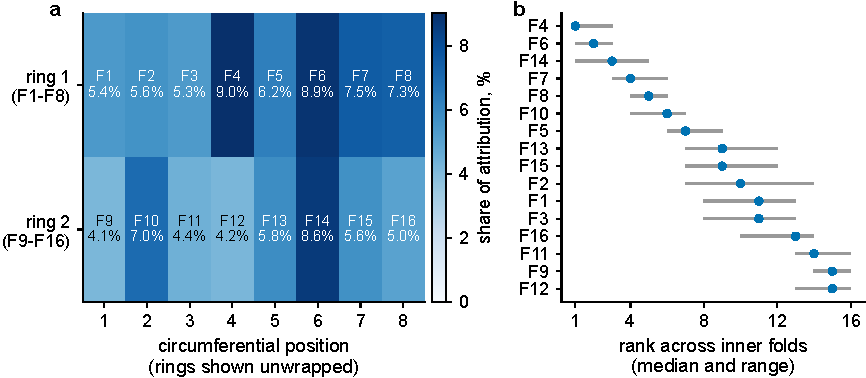
\includegraphics[width=\textwidth]{figures/fig7_attribution.pdf}
\caption{Cross-fitted electrode attribution on GRABMyo ($\lambda = 0$, 43 outer folds). (a) Mean share of attribution per electrode, drawn on the $2 \times 8$ montage; each ring~2 electrode is aligned with, and 2~cm from, the ring~1 electrode at the same circumferential position. (b) Rank of each electrode across inner folds (median and range).}
\label{fig:attribution}
\end{figure}

Replication on NinaPro DB5 was inconclusive. The dataset contained only ten participants and produced substantially wider uncertainty than GRABMyo: full-array Macro-F1 was \DBFiveFull\ $\pm$ \DBFiveFullSD\ (12 movements; chance about 0.083), with between-subject values from \DBFiveFullMin\ to \DBFiveFullMax\ (figure~\ref{fig:generalisation}(b); supplementary table~S8). One reduced configuration ($k = 12$) met the non-inferiority margin by a negligible amount ($\bar\Delta_{12} = \DBFiveDeltaKTwelve$, lower bound $\DBFiveDeltaKTwelveLCBSix$), but the decision was sensitive to Monte Carlo variation in the bootstrap: it was non-inferior in \DBFiveSeedHits\ of \DBFiveSeedN\ bootstrap reruns with different random seeds (\DBFiveSeedFrac\%), a decision-stability diagnostic rather than a probability that the hypothesis is true. Subsets with $k = 13$, 14 and 15 all failed (lower bounds $\DBFiveDeltaKThirteenLCB$, $\DBFiveDeltaKFourteenLCB$ and $\DBFiveDeltaKFifteenLCB$), and no subset remained non-inferior after Holm correction. The replication therefore neither confirms nor contradicts the primary GRABMyo result.

Cross-session analyses provided no evidence of an additional performance loss on later recording days beyond the existing subject-independent gap (figure~\ref{fig:generalisation}(a); supplementary table~S9). Training on session~1 and testing on sessions 1, 2 and 3 gave \CSOneSOne, \CSOneSTwo\ and \CSOneSThree; \chg{session~2 scored higher than session~1} ($\CSSTwoVsSOneDiff$, 95\% CI $\CSSTwoVsSOneLCB$ to $\CSSTwoVsSOneUCB$, uncorrected $p \CSSTwoVsSOneP$), and no statistically detectable difference was observed for session~3 ($\CSSThreeVsSOneDiff$, $p \CSSThreeVsSOneP$). Training on sessions 1 and 2 improved session-3 performance over training on session~1 alone ($\CSTwoVsOneDiff$, 95\% CI $\CSTwoVsOneLCB$ to $\CSTwoVsOneUCB$, $p \CSTwoVsOneP$). However, these contrasts do not isolate electrode displacement, and the apparent benefit of training on two sessions is confounded by the larger amount of training data.

Finally, results from the derived bipolar representation differed from those of the primary monopolar analysis. With the eight derived pairs as the selection unit, full-array Macro-F1 was \BipFull\ $\pm$ \BipFullSD\ for a model trained on all training windows, lower than \chg{the monopolar full-array result} (figure~\ref{fig:generalisation}(c)). As in the monopolar analysis, the reduction curve used a 200,000-window training sample; its $k = 8$ reference scored \BipCurveRefK\ (supplementary table~S10). \chg{The reduction from eight to seven bipolar pairs did not satisfy} the primary non-inferiority criterion ($\bar\Delta_7 = \BipDeltaKSeven$, lower bound $\BipDeltaKSevenLCB$; non-inferior in \BipSeedHitsSeven\ of \BipSeedN\ bootstrap reruns). Under the sensitivity margins, $k^*$ was \BipKStarMarginPtOne\ at $\delta = 0.01$ and \BipKStarMarginPtThree\ at $\delta = 0.03$, identically for all $\lambda$, and pairs \BipTopThreeSet\ formed the top three in \BipTopThreeFolds\ of 43 folds. Consequently, the \KStarReductionPct\% reduction identified in the primary analysis should be interpreted specifically as a reduction in monopolar recording sites on the GRABMyo montage, rather than as evidence that an equivalent proportion of physical bipolar sensors can be removed.

\begin{figure}[t]
\centering
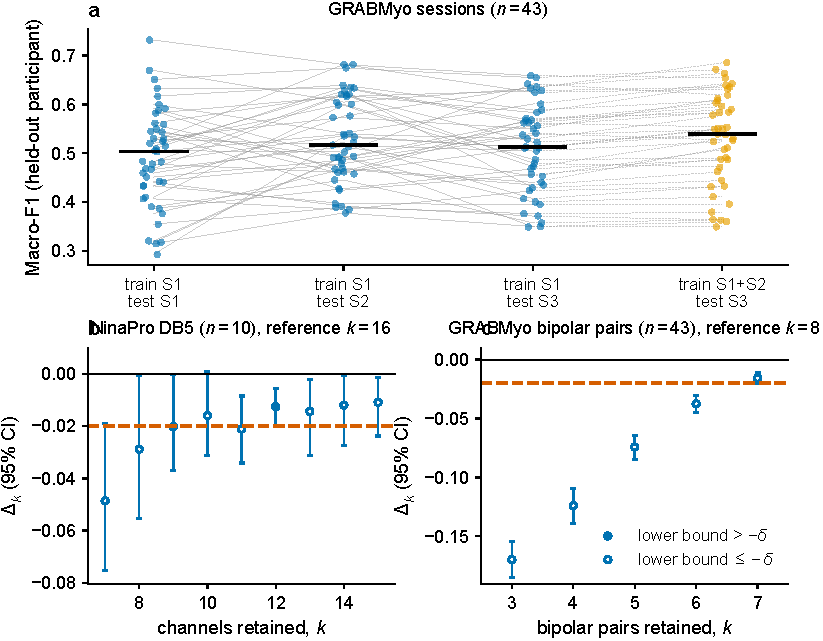
\includegraphics[width=\textwidth]{figures/fig8_generalisation.pdf}
\caption{Exploratory analyses. (a) GRABMyo cross-session evaluation: each point is one held-out participant, grey lines join the same participant across conditions and bars mark medians; every condition is also subject-independent. (b--c) Mean paired difference to the full array of the same curve, $\bar\Delta_k$, with 95\% cluster-bootstrap confidence interval, for (b) NinaPro DB5 (10 subjects, reference $k = 16$), (c) GRABMyo derived bipolar pairs (43 participants, reference $k = 8$). The dashed line marks the primary margin; filled markers indicate a lower bound above the margin and open markers a lower bound at or below it.}
\label{fig:generalisation}
\end{figure}

\needspace{8\baselineskip}
\section{Discussion}
\label{sec:discussion}

This study examined how far a 16-electrode forearm sEMG array could be reduced while preserving subject-independent gesture-recognition performance under a prespecified engineering tolerance. The principal finding was a moderate reduction: four electrodes could be removed \chg{within the margin, whereas removing five did not meet the criterion.} The smallest non-inferior configuration therefore contained \KStar\ electrodes, representing a \KStarReductionPct\% reduction from the complete array. This result was not driven by a single irregular point on the performance curve: all configurations from 12 to 15 electrodes remained within the non-inferiority margin, and the minimum acceptable count was unchanged after correction for multiple testing. At the same time, every reduction produced some numerical loss in Macro-F1, and halving the array incurred a substantially larger decrease. The full montage therefore contains some redundancy, \chg{although less than user-dependent electrode-selection studies might suggest.}

This distinction between user-dependent and subject-independent reduction is central to the interpretation of the result. A sparse configuration optimised for a particular individual can exploit that person's anatomy, electrode placement and activation patterns. A layout intended for previously unseen users must instead preserve information across inter-individual variability. The present result \chg{should therefore not} be interpreted as contradicting studies reporting successful control with substantially fewer electrodes \citep{phinyomark2018emg,qu2021reduce}; rather, it addresses a different design question. Under the current montage, gesture set and cross-user protocol, a moderate reduction was supported, whereas larger reductions in electrode count were not.

Cross-fitted attribution provided useful information for selecting which electrodes to retain, but its benefit was more limited than a comparison with random subsets alone might suggest. Both attribution rankings outperformed the mean random-subset baseline at every tested subset size, and deletion with retraining showed that removing highly ranked electrodes was more damaging than removing weakly ranked ones. Together, these findings support the functional relevance of the ranking. However, the attribution-based configuration was rarely among the highest-scoring random subsets for an individual participant, and exploratory comparisons showed no statistically detectable advantage over permutation importance or an evenly spaced geometric layout at most tested subset sizes. The clearest separation occurred at six electrodes, where the attribution-guided ranking scored higher than both the geometric layout and permutation importance in uncorrected exploratory contrasts.

This pattern suggests that two effects may be operating simultaneously. The forearm montage appears to contain broad spatial redundancy, making circumferential coverage an effective baseline when a relatively large number of electrodes is retained. At six electrodes, the identity of individual recording locations appeared to matter more. No advantage over the geometric layout was detected at four electrodes, however, so the benefit of attribution did not simply increase as the array was reduced. This interpretation remains exploratory: the study did not formally test equivalence between attribution-based and geometric layouts, nor did it test whether the geometric layout itself satisfies the non-inferiority criterion. The absence of a statistically detectable difference should therefore not be interpreted as evidence that the two approaches are interchangeable.

Stability regularisation provided no statistically detectable benefit. The cross-fitted attribution profiles were already highly similar across inner participant groups, leaving little instability for the regularisation term to penalise; the penalty changed the top-12 set in at most one of 43 folds. Consequently, the stability-adjusted rankings were almost identical to the rankings based on attribution magnitude alone. The post-hoc participant-level extension made between-person variability more visible but reached the same practical conclusion: a more sensitive estimate of attribution heterogeneity did not translate into improved electrode selection. Within the present dataset and sample size, the tested stability formulation added no detectable ranking information beyond \chg{cross-fitted TreeSHAP magnitude alone}, suggesting that the additional stability term was unnecessary under the present protocol. This result does not exclude a role for stability regularisation \citep{xiang2026roshap} in smaller cohorts, more heterogeneous populations, or settings in which attribution estimates vary more strongly across participants.

The spatial consistency of the ranking also warrants careful interpretation. Several electrode positions were repeatedly ranked near the top across outer folds and individual participants, indicating reproducible regional differences in discriminative information. However, these positions cannot be interpreted directly as specific muscle contributions. \chg{GRABMyo documents the electrode positions but not the underlying muscle boundaries}, no imaging-based electrode-to-muscle registration was available, and each surface recording reflects volume-conducted activity from multiple sources \citep{farina2004extraction}. The present results therefore support a positional interpretation (some circumferential regions are consistently more informative than others) but not muscle-level localisation.

The exploratory analyses further define the scope of the primary result. NinaPro DB5 did not provide a decisive external replication because its ten participants yielded wide uncertainty and the candidate non-inferior configuration did not survive multiplicity correction. Similarly, the cross-session analysis did not reveal an additional performance penalty on later recording days, but this should not be interpreted as evidence that electrode displacement or repeated donning is inconsequential \citep{hargrove2006effect,kaufmann2010fluctuating,vidovic2016improving}. All conditions remained subject-independent, and training on multiple sessions also increased the amount of available training data. Most importantly, the bipolar re-referencing analysis did not reproduce the degree of reduction observed for monopolar electrodes: removing even one of eight derived bipolar pairs failed the primary non-inferiority criterion. The observed \KStarReductionPct\% reduction is therefore specific to monopolar recording sites on the analysed two-ring montage and should not be translated directly into a claim about reducing physical bipolar sensors.

Several limitations constrain the generality of these findings. The primary LOSO analysis evaluates the reduction procedure and the electrode count it supports within the available cohort; it does not constitute an independent prospective validation of a fixed sparse hardware layout. The same four electrodes were excluded at $k = 12$ in \DroppedFourFolds\ of 43 folds, but \chg{one frozen layout was tested only in two single-split checks (supplementary methods~S4). The layout met the non-inferiority criterion in one split direction and missed it narrowly in the other (lower bound $\FixedSwapLCBSix$), and the electrode count had been chosen after the full-cohort curve was inspected.} All participants were able-bodied, and the analysis was entirely offline. Zero-phase filtering is non-causal, and the present evaluation therefore does not establish real-time control performance. Effects of fatigue, posture, electrode displacement and repeated donning were not isolated. The electrode rankings were derived from models trained on the complete array and may differ from rankings learned directly under sparse acquisition. Computational constraints also required reduced training samples for some classifier and selection-method comparisons: the support vector machine result is therefore likely a lower bound, and the H2 and H4 comparisons used a lighter model than the performance curve. Training-sample sizes were chosen on two folds using held-out outcomes, and $\lambda$ was not selected. In addition, the detailed secondary test families and several exploratory analyses were specified after the primary results were available, as documented in supplementary methods~S1, and should be interpreted accordingly; the window-length and 17-class analyses listed in the plan were not run. Finally, the independent replication dataset was small, and the bipolar analysis used signals derived mathematically from monopolar recordings rather than measurements from a physical bipolar montage.

Taken together, the findings support a restrained design conclusion rather than a claim for extensive electrode reduction. For subject-independent recognition, the relevant question is not whether some sparse configuration can perform well for particular users, but whether the performance loss associated with a common reduced configuration remains within a tolerance defined before observing the result. Under that criterion, this study supports a moderate reduction from 16 to 12 monopolar electrodes. Cross-fitted attribution offers a leakage-controlled way to identify informative sites, but its practical advantage depends on how strongly the array is reduced and may be modest when broad spatial coverage is already preserved.

\section{Conclusion}
\label{sec:conclusion}

For offline, subject-independent gesture recognition with the two-ring monopolar GRABMyo montage, a subset of \KStar\ of 16 electrodes satisfied the prespecified non-inferiority criterion (margin 0.02 Macro-F1), whereas 11 electrodes did not; the evidence therefore supports a moderate rather than an extensive reduction. Cross-fitted attribution outperformed the mean random-subset baseline at each tested subset size, and deletion with retraining supported the functional relevance of the ranking, but its advantage over simple spatial selection was limited to one of the tested subset sizes in exploratory comparisons. Stability regularisation added no statistically detectable benefit under the present protocol. Because the analysis evaluated a selection procedure within one offline cohort and montage, independent validation of a fixed sparse hardware layout, in target clinical populations and in online causal control, remains necessary before deployment recommendations can be made.


\ack{[AUTHOR INPUT REQUIRED: acknowledgements, if any.]}

\funding{[AUTHOR INPUT REQUIRED: funding source and grant number, or `This research received no specific grant from any funding agency in the public, commercial or not-for-profit sectors.' only if true.]}

\roles{[AUTHOR INPUT REQUIRED: contributions of Minh-Tri Ta, Hoang-Khang Phan and Le-Giang Tran using CRediT roles.]}

\section*{Conflict of interest}
[AUTHOR INPUT REQUIRED: confirm the conflict-of-interest declaration.]

\data{GRABMyo v1.1.0 is available from PhysioNet \citep{jiang2024grabmyo} (\url{https://doi.org/10.13026/89dm-f662}); NinaPro DB5 from the NinaPro repository (\url{https://ninapro.hevs.ch}). The statistical analysis plan, the record of analysis decisions, the analysis code, the environment specification and all result files from which the numbers in this paper are computed are archived at [AUTHOR INPUT REQUIRED: INSERT PERMANENT REPOSITORY DOI].}

\suppdata{Supplementary methods S1--S6 (departures from the analysis plan, threshold checks, deletion-analysis consistency, the fixed-layout consistency check, feature redundancy and the participant-level attribution extension), supplementary tables S1--S10 and supplementary figures S1--S2 are provided in a separate file.}

\bibliographystyle{jphysicsB}
\bibliography{references}

\end{document}
